\chapter{Resultados}
\label{chap:resultados}

% Referencias a documentos externos
\externaldocument{metodo}

\drop{E}{n} este capítulo se muestran los resultados obtenidos para la consecución del presente \ac{TFG}. La estructura del capítulo se basa en las iteraciones propias de la metodología elegida y definida en la sección 4 (ver sección \ref{section:desarrollo}). Es necesario llevar a cabo un sprint 0 que servirá para detallar los apartados principales de la gestión del mismo, como los requisitos y el alcance del proyecto, las historias de usuario, la gestión temporal, gestión de usuarios y riesgos y otras acciones necesarias.

Debido al carácter académico del proyecto, los recursos y la gestión de los mismos estarán alejados de los parámetros habituales del mercado laboral, ya que todos los roles necesarios serán desarrollados por dos personas, el autor y el director del proyecto.

\section{Sprint 0}
Esta primera iteración tiene como objetivo definir el alcance del proyecto y su realizar la planificación del mismo, de manera que quede definida una sólida base sobre la que comenzar el desarrollo del mismo. Se estimará el coste temporal y económico, y se abordará la planificación de los recursos que se consideran necesarios para la correcta consecución de los objetivos planteados, tanto técnicos como humanos, y la gestión de los mismos que se pretende llevar a cabo.

	\subsection{Gestión de recursos humanos}
	Tal y como se comentó en la introducción al capítulo, las personas involucradas en el desarrollo del proyecto son el autor y el director del mismo, que coparán todos los roles disponibles, quedando estos de la siguiente manera:
	
	\begin{itemize}[label={$\bullet$},labelindent=\parindent,leftmargin=2cm]
		\item Autor del \ac{TFG}: Equipo de desarrollo, análisis y pruebas del producto.
		\item Director del \ac{TFG}: Propietario, usuario y cliente final del producto.
	\end{itemize}
	
	\subsection{Alcance del proyecto}
		\subsubsection{Descripción del alcance}
		\label{subsubsection:descripcion-alcance}
		El proyecto consistirá en la elaboración de una herramienta accesible a través de una página web, asimismo se proporcionará una aplicación móvil para sistemas operativos Android que facilitará el acceso a la mencionada página.
		\\La página constará de dos secciones delimitadas por los privilegios necesarios de acceso. 
		
		Una primera sección de acceso libre en la que se encuadran las páginas \textit{Inicio}, \textit{Acerca de}, \textit{Contacto} y aquellas páginas auxiliares necesarias para permitir el registro y autenticación a los usuarios que deseen acceder a la segunda sección.
		\\Para ganar acceso a la segunda sección será necesario autentificarse mediante un usuario y una contraseña adquiridos mediante un formulario de registro. Esta sección englobará las páginas de gestión de los datos personales del usuario y el acceso a las posiciones geográficas guardadas para este usuario.
		\\La herramienta permitirá al usuario definir una localización geográfica como posición de aparcamiento de su vehículo seleccionando la ubicación mediante un mapa interactivo.
		La herramienta mostrará al usuario la localización actual de los elementos guardados previamente mediante un mapa interactivo.
		\\Los usuarios podrán permitir la compartición de la localización de un elemento con otros usuarios legítimos de la herramienta, llamados \textit{usuarios secundarios}.
		\\Los \textit{usuarios secundarios} podrán modificar los elementos compartidos bajo las mismas condiciones que el \textit{usuario primario} o usuario propietario del elemento.
		\\El \textit{usuario primario} podrá revocar los derechos de acceso y edición a los \textit{usuarios secundarios}.
		La herramienta estará diseñada para facilitar el acceso a través de dispositivos móviles mediante los navegadores incorporados.
		\\Se pondrá a disposición de los usuarios con sistemas operativos Android una aplicación que permitirá el acceso rápido a la herramienta web.
	
		\subsubsection{Criterios de aceptación}
		\label{subsubsection:criterios-aceptacion}
		La herramienta se considerará conforme a criterio siempre que cumpla los puntos detallados a continuación.
		
		\begin{itemize}[label={$\bullet$},labelindent=\parindent,leftmargin=2cm]
			\item La herramienta web debe visualizarse correctamente en los navegadores Midori, Chromium,Chrome y Mozilla Firefox.
			\item La aplicación debe dar acceso a la herramienta web y permitir una correcta visualización de la misma.
			\item La herramienta web debe garantizar el acceso mediante autenticación a los usuarios legítimos, impidiendo el acceso a la sección restringida a los usuarios no identificados.
			\item La herramienta web debe contener mecanismos para el alta de nuevos usuarios y contendrá mecanismos para la recuperación de los datos de entrada por parte de los usuarios legítimos.
			\item La herramienta mostrará un mapa interactivo en el que estarán señalados los elementos guardados por el usuario y permitirá la adición de nuevos elementos o la modificación de los existentes.
			\item La herramienta incorporará mecanismos para permitir la compartición de elementos entre usuarios legítimos y para revocar está compartición.
			\item La herramienta permitirá a los \textit{usuarios secundarios} modificar los elementos compartidos con ellos por los \textit{usuarios primarios}.
			\item La herramienta permitirá a los \textit{usuarios primarios} revocar los derechos de visión y edición de los \textit{usuarios secundarios} a los elementos previamente compartidos.
			\item La aplicación estará desplegada en un servidor accesible a cualquier usuario con acceso a internet.
			\item La herramienta será accesible a través de una aplicación móvil para sistemas operativos Android.
		\end{itemize}

		\subsubsection{Entregables del proyecto}
		Al finalizar cada una de las iteraciones se entregará al cliente un artefacto en forma de página de web con las características añadidas a la herramienta durante la iteración así como la documentación generada durante esta fase.
		
	Al termino de las iteraciones se entregará la herramienta completa según lo descrito en la descripción del alcance (ver descripción del alcance \ref{subsubsection:descripcion-alcance}) conforme a criterios (ver criterios \ref{subsubsection:criterios-aceptacion}), un manual de usuario de la herramienta, un manual de instalación, una aplicación móvil y una memoria con los documentos generados durante el proceso de desarrollo.
	
		\subsubsection{Suposiciones y restricciones del proyecto}
		Para asegurar el correcto funcionamiento de la herramienta debe tenerse en cuenta los puntos descritos a continuación:
		
		\begin{itemize}[label={$\bullet$},labelindent=\parindent,leftmargin=2cm]
			\item Se asegura el correcto funcionamiento al acceder desde los siguientes navegadores: Midori, Chromium, Chrome y Mozilla Firefox.
			\item La aplicación móvil será compatible con versiones Android 4.1 y posteriores.
		\end{itemize}

	\subsection{Plan del proyecto}
	En función de los requisitos del proyecto, definidos en la sección \textit{Objetivos} \ref{chap:objetivos} y teniendo en cuenta el alcance del proyecto (ver subsección \ref{subsubsection:descripcion-alcance}) y los criterios de aceptación del mismo (ver subsección \ref{subsubsection:criterios-aceptacion}) se puede crear la pila de producto, que consistirá en una colección de \textit{historias de usuario} del sistema, su valor de negocio y la estimación temporal para llevarlo a cabo. Tanto el valor de negocio como la estimación han sido llevadas a cabo contando con la ayuda del propietario del producto.
	En la tabla \ref{tab:historia_usuario} podemos observar las historias de usuario retratadas en una pila de producto priorizada en la que se incluye una estimación temporal y el valor de negocio considerado para la misma.


	\begin{longtable}{p{2cm} p{6cm} p{4cm} p{3cm}}
	  	\hline
  	    \multicolumn{1}{p{2cm}}{\cellcolor{black!30}\textbf{Id}} &
	    \multicolumn{1}{p{6cm}}{\cellcolor{black!30}\textbf{Historia de Usuario}} & 
	 	\multicolumn{1}{p{4cm}}{\cellcolor{black!30}\textbf{Estimación temporal}} &
 	 	\multicolumn{1}{p{3cm}}{\cellcolor{black!30}\textbf{Valor de negocio}}
	 	\\
	 	\toprule 
	   % \toprule
	   	\endfirsthead
	     
	    \hline
  	    \multicolumn{1}{p{2cm}}{\cellcolor{black!30}\textbf{Id}} &
	    \multicolumn{1}{p{6cm}}{\cellcolor{black!30}\textbf{Historia de Usuario}} & 
	 	\multicolumn{1}{p{4cm}}{\cellcolor{black!30}\textbf{Estimación temporal}} &
 	 	\multicolumn{1}{p{3cm}}{\cellcolor{black!30}\textbf{Valor de negocio}}
	 	\\	 
	 	\toprule
	 	\endhead	

		\rowcolor{gray!25}
		HdU 1	&	Como cliente quiero que los usuarios se registren antes de acceder a la aplicación y a sus datos	
				&	20 horas		&	Alto	\\
		HdU 2	&	Como usuario quiero acceder mediante un nombre y una contraseña para que sólo yo pueda entrar a mi cuenta							&	10 horas	&	Alto	\\
		\rowcolor{gray!25}
		HdU 3	&	Como usuario quiero modificar mis datos guardados	o eliminar mi cuenta												
				&	12 horas	&	Alto	\\ 
		HdU 4	& 	Como usuario quiero guardar mis ubicaciones mediante un mapa para poder acceder a ellas más tarde	
				&	30 horas	&	Alto	\\
		\rowcolor{gray!25}
		HdU 5	&	Como usuario quiero recuperar todas mis ubicaciones guardadas, verlas dibujadas en un mapa y ver el nombre y el número de la calle donde están aparcados
				&	12 horas	&	Alto	\\
		HdU 6	&	Como usuario quiero recuperar y ver en el mapa una de mis ubicaciones guardadas, también quiero ver la dirección postal completa
				&	10 horas	&	Alto	\\
		\rowcolor{gray!25}
		HdU 7	&	Como usuario quiero poder añadir mis coches para poder guardar su ubicación															&	12 horas	&	Alto	\\
		HdU 8	&	Como usuario quiero poder borrar o editar los datos guardados de mis coches
				&	12 horas	&	Medio	\\	
		\rowcolor{gray!25}
		HdU 9	&	Como usuario quiero compartir mis ubicaciones guardadas con otros usuarios de mi elección para que puedan modificarlas			
				&	30 horas&	Medio	\\
		HdU 10	&	Como usuario quiero dejar de compartir mis ubicaciones guardadas con otros usuarios de mi elección para que puedan modificarlas			
				&	10 horas&	Medio	\\
		\rowcolor{gray!25}
		HdU 11	&	Como usuario quiero que la aplicación me muestre la ruta a pie desde mi posición actual hasta la ubicación seleccionada
				&	6 horas	&	Bajo	\\
		HdU 12	&	Como usuario quiero poder acceder a la herramienta a través de una aplicación instalada en mi móvil
				&	6 horas	&	Bajo	\\
	    \hline
	  \caption{Objetivos parciales del \ac{TFG}}
	  \label{tab:historia_usuario}
	\end{longtable}

Una vez tenemos la lista de producto priorizada podemos dividir el trabajo en los distintos sprint que generarán como resultado la consecución de los objetivos marcados. En las tablas \ref{tab:plan_proyecto} y \ref{tab:validaciones_HdU} podemos observar la división realizada, los artefactos resultantes y la validación necesaria para lograr el objetivo marcado.

\begin{longtable}{p{1cm} p{4cm} p{4cm} p{6cm}}
  	\hline  	    
  	\multicolumn{1}{p{1cm}}{\cellcolor{black!30}\textbf{Sprint}} &
    \multicolumn{1}{p{4cm}}{\cellcolor{black!30}\textbf{Historia de Usuario}} & 
 	\multicolumn{1}{p{4cm}}{\cellcolor{black!30}\textbf{Estimación temporal}} &
 	\multicolumn{1}{p{6cm}}{\cellcolor{black!30}\textbf{Artefactos}}
 	\\
 	\toprule 
   % \toprule
   	\endfirsthead
     
    \hline
  	\multicolumn{1}{p{1cm}}{\cellcolor{black!30}\textbf{Sprint}} &
    \multicolumn{1}{p{4cm}}{\cellcolor{black!30}\textbf{Historia de Usuario}} & 
 	\multicolumn{1}{p{4cm}}{\cellcolor{black!30}\textbf{Estimación temporal}} &
 	\multicolumn{1}{p{6cm}}{\cellcolor{black!30}\textbf{Artefactos}}
 	\\	 
 	\toprule
 	\endhead

	\rowcolor{gray!25}
	1	& HdU 1, HdU 2 y HdU 3	&	42 horas	&	Prototipo de página web con autenticación, edición y administración de usuarios \\ 
	2	& HdU 5					&	12 horas	&	Prototipo que muestre en un mapa una serie de ubicaciones geográficas guardadas previamente y sus correspondientes direcciones postales mediante un texto \\
	\rowcolor{gray!25}
	3	& HdU 4				&	30 horas	&	Prototipo que guarde una ubicación geográfica elegida por el usuario mediante la interacción con un mapa \\
	4	& HdU 7					&	12 horas	&	Prototipo que permite crear nuevos elementos para almacenar la ubicación geográfica del mismo y muestra la ubicación de un elemento seleccionado \\
	\rowcolor{gray!25}
	5	& HdU 6					& 	10 horas	& 	Prototipo que muestra en un mapa la posición de un elemento seleccionado y su correspondiente dirección postal mediante texto\\
	6	& HdU 8					&	12 horas	&	Prototipo que permite modificar o borrar los datos almacenados de los elementos a mostrar \\
	\rowcolor{gray!25}
	7	& HdU 9 y HdU 10		&	40 horas	&	Prototipo que permite compartir la ubicación de los elementos almacenados con otros usuarios válidos del sistema y revocar este permiso \\
	8	& HdU 11				&	6 horas		&	Prototipo que muestra la ruta a pie desde la posición actual del usuario hasta el elemento seleccionado \\
	\rowcolor{gray!25}
	9	& HdU 12				&	6 horas		&	Prototipo que permite el acceso a la herramienta a través de una aplicación instalada en dispositivos móviles \\
	\hline
	\caption{Plan de proyecto detallado}
	\label{tab:plan_proyecto}
\end{longtable}

\begin{longtable}{p{1cm} p{4cm} p{4cm} p{6cm}}
  	\hline  	    
  	\multicolumn{1}{p{1cm}}{\cellcolor{black!30}\textbf{Sprint}} &
    \multicolumn{1}{p{4cm}}{\cellcolor{black!30}\textbf{Historia de Usuario}} & 
 	\multicolumn{1}{p{4cm}}{\cellcolor{black!30}\textbf{Estimación temporal}} &
 	\multicolumn{1}{p{6cm}}{\cellcolor{black!30}\textbf{Validación}}
 	\\
 	\toprule 
   	\endfirsthead
	%\multirow{3}{4cm}{multifila 1-3} &
	     
    \hline
  	\multicolumn{1}{p{1cm}}{\cellcolor{black!30}\textbf{Sprint}} &
    \multicolumn{1}{p{4cm}}{\cellcolor{black!30}\textbf{Historia de Usuario}} & 
 	\multicolumn{1}{p{4cm}}{\cellcolor{black!30}\textbf{Estimación temporal}} &
 	\multicolumn{1}{p{6cm}}{\cellcolor{black!30}\textbf{Validación}}
 	\\	 
 	\toprule
 	\endhead

	\rowcolor{gray!25}
	\multirow{3}{*}{1}	& HdU 1	&	20 horas	&	Los usuarios anónimos pueden darse de alta en el sistema. \\ 
	\rowcolor{gray!25}	& HdU 2	&	10 horas	&	Los usuarios anónimos no pueden acceder a la aplicación. Los usuarios registrados 														pueden acceder a la aplicación. \\ 
	\rowcolor{gray!25}	& HdU 3	&	12 horas	&	Los usuarios registrados pueden modificar los datos de su cuenta o darse de baja en 														la aplicación.  \\                      
	
	2	& HdU 5		&	12 horas	&	Los usuarios registrados podrán ver en un mapa las ubicaciones guardadas y en un cuadro de 												texto la dirección postal de la misma.\\
	\rowcolor{gray!25}
	3	& HdU 4		&	30 horas	&	Los usuarios registrados podrán guardar en la base de datos ubicaciones 																	interactuando con el mapa. \\
	
	4	& HdU 7		&	12 horas	&	Los usuarios registrados podrán crear nuevos elementos sobre los que guardar ubicaciones 													geográficas. \\
	\rowcolor{gray!25}
	5	& HdU 6		&	10 horas	&	Los usuarios registrados podrán seleccionar uno de los elementos 																			guardados para mostrar únicamente su ubicación en el mapa. \\

	6	& HdU 8		&	12 horas	&	Los usuarios registrados podrán modificar las propiedades de los elementos que hayan creado o 											borrarlos del sistema. \\
	\rowcolor{gray!25}
	\multirow{2}{*}{7}	& HdU 9		&	30 horas	&	Los usuarios registrados podrán ver y modificar las ubicaciones de los elementos 															previamente compartidos con ellos por otros usuarios registrados. \\
	\rowcolor{gray!25}	& HdU 10	&	10 horas	&	Los usuarios registrados no podrán ver ni modificar las ubicaciones de los 																elementos que hayan dejado de compartirse con ellos por otros usuarios 																	registrados. \\

	8	& HdU 11	&	6 horas		&	Los usuarios registrados podrán ver una ruta a pie desde su ubicación actual hasta la ubicación 											almacenada del elemento seleccionado. \\

	\rowcolor{gray!25}
	9	& HdU 12	&	6 horas		&	Los usuarios podrán acceder a la herramienta usando una aplicación instalada en sus dispositivos móviles. \\
	\hline
	\caption{Historias de Usuario y validaciones}
	\label{tab:validaciones_HdU}
\end{longtable}

	\subsection{Gestión temporal del proyecto}
	Una vez definido el alcance del proyecto mediante las historias de usuario y su división en sprint, se realizará un diagrama de Gantt con la estimación temporal del proyecto.
	Como fecha de inicio para el desarrollo, esto es, para el sprint 0 se elige la fecha de 15 de septiembre de 2015 y para la consecución del mismo se estima una duración aproximada de veinticuatro días. La duración de la jornada laboral se fija en 6 horas diarias de lunes a viernes, observando las fechas marcadas como festivo en el calendario laboral general.
	Debido a que el equipo de desarrollo está formado por una única persona, la posibilidad de paralelizar trabajo se ve limitada a la elaboración de la presente memoria al tiempo que se realiza el desarrollo de la aplicación, pero no al desarrollo de historias de usuario simultáneamente.
	Se estima que la realización, revisión y corrección de la memoria necesitará un tiempo total de trabajo de quince días aproximadamente.
	En la figura \ref{fig:gantt} puede observarse el correspondiente diagrama de Gantt de la planificación.

\begin{sidewaysfigure}[h!t]
	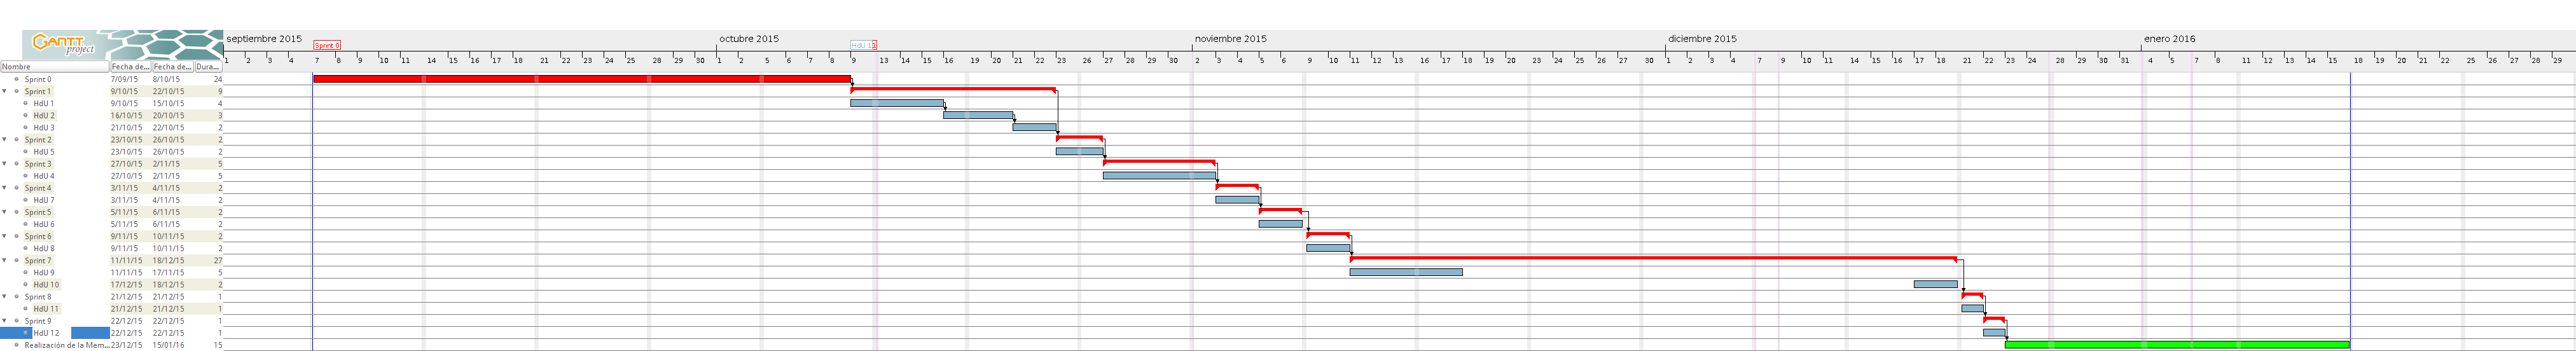
\includegraphics[height=80mm, fbox={\fboxrule} 4mm]{./images/05-resultados/01-gantt.png}
	\caption{Diagrama de Gantt del \ac{TFG}}
	\label{fig:gantt}
\end{sidewaysfigure}
	
	\subsection{Gestión de las comunicaciones}
	La comunicación entre el autor del presente \ac{TFG} y el director del proyecto se realizará para la información puntual del estado del desarrollo y abordar las posibles dudas generadas durante el desarrollo. Generalmente las reuniones se realizarán semanalmente y se concretarán, preferentemente, mediante correo electrónico.
	Se utilizarán también otro tipo de herramientas para comunicar en todo momento el estado del proyecto y facilitar la comunicación entre los dos actores principales del desarrollo, a saber, el autor y el director. Estas herramientas serán \textit{Trello}, \textit{Github} y \textit{Heroku}.\\
	Trello, tal y como se explicó anteriormente (ver subsección \ref{subsubsection:trello}) es un tablero Kanban virtual que permitirá al director estar informado en todo momento de las tareas que el autor está llevando a cabo en cada momento, así como la modificación de la lista de tareas si así lo considerase necesario. Para ello se crea y permite el acceso al director a un nuevo tablero Kanban iniciado para el presente proyecto. En la figura \ref{fig:trello} puede observarse una captura de pantalla del panel Kanban en Trello.

\begin{figure}[H]
\centering
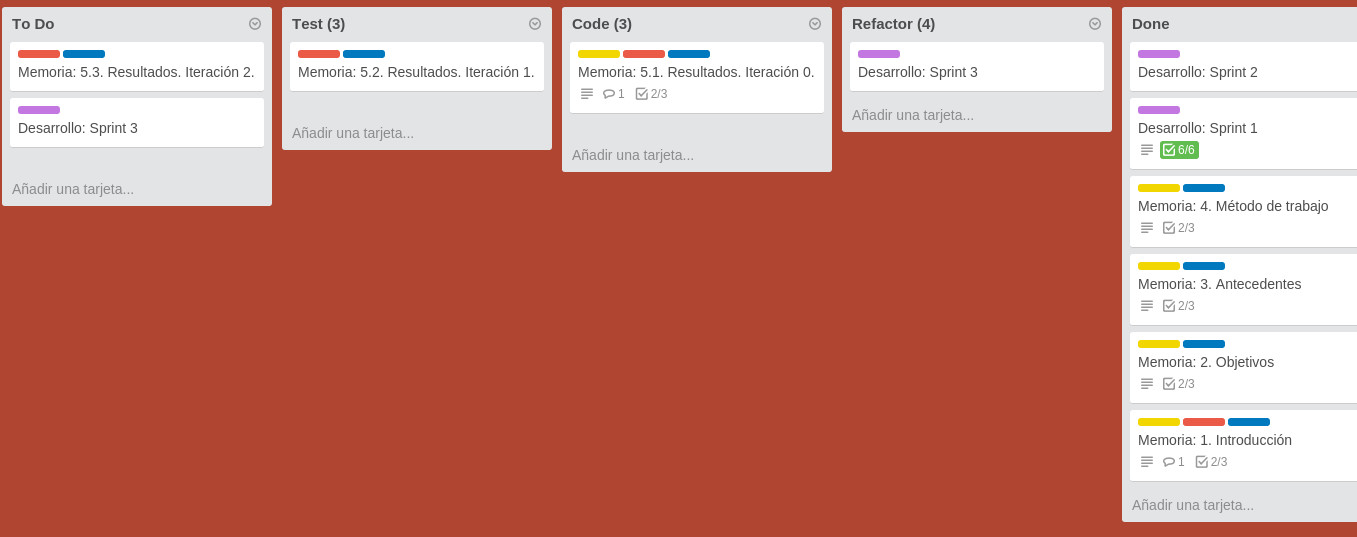
\includegraphics[width=15cm, fbox={\fboxrule} 4mm]{images/05-resultados/03-trello.jpg}
\caption{Panel Kamban de Trello}
\label{fig:trello}
\end{figure}
	
	
	Github, tal y como se explicó anteriormente (ver subsección \ref{subsubsection:github}) es un servidor para repositorios \textit{Git} que se utilizará para el almacenaje en línea tanto del código del proyecto como de la memoria del mismo. Debido a las restricciones existentes en el servicio gratuito, el repositorio es público, por lo que únicamente se procederá a informar al director del proyecto de la dirección donde se encuentra almacenado. Mediante estos actos, se conseguirá que el director tenga acceso completo a toda la documentación generada para la consecución del proyecto pudiendo revisarla cuando así lo que creyera necesario. Esto mismo es aplicable al código fuente del presente proyecto. En la figura \ref{fig:github} puede verse una captura de pantalla de algunos commit subidos al repositorio.
	
\begin{figure}[H]
\centering
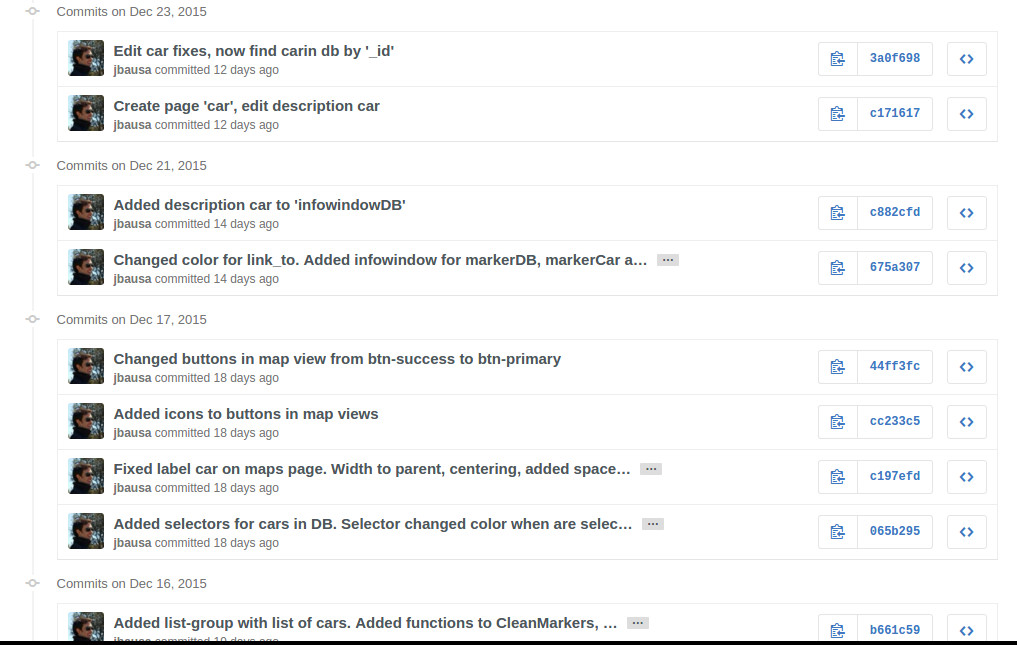
\includegraphics[width=15cm, fbox={\fboxrule} 4mm]{images/05-resultados/02-git.jpg}
\caption{Commits en repositorio en GitHub}
\label{fig:github}
\end{figure}
	
	Heroku, tal y como se explicó anteriormente (ver subsección \ref{subsubsection:heroku}) es el servidor usado para la implantación del presente proyecto, por lo que se utilizará para comprobar los avances en el proyecto mediante la visita a través de un navegador web.
	
	\subsection{Gestión de recursos}
	Tal y como se comentó anteriormente (ver sección \ref{section:dispositivos-empleados}), para el desarrollo del proyecto se utilizará un equipo con las características detalladas en la tabla \ref{tab:portatil2}. 
	
	\begin{table}[H]
	  \centering 
	  \rowcolors{1}{gray!25}{white}
	  \begin{tabular}{p{0.4\linewidth}p{0.3\linewidth}}
	    \toprule
		Procesador 							& Intel i7-5500U								\\
		Velocidad y Núcleos del Procesador & 2.4 GHz; 2 núcleos 							\\
		Memoria RAM 						& 16 \ac{GB} \ac{DDR}3L \ac{SDRAM} 			\\
		Sistema Operativo					& Elementary \ac{OS} 							\\
	    \hline
	  \end{tabular}
	  \caption{Equipo usado para el desarrollo \ac{TFG}}
	  \label{tab:portatil2}
	\end{table}
	
	Para las pruebas con dispositivos móviles se utilizará un equipo con las características mostradas en la tabla \ref{tab:movil2}.
	\begin{table}[H]
	  \centering 
	  \rowcolors{1}{gray!25}{white}
	  \begin{tabular}{p{0.3\linewidth}p{0.4\linewidth}}
	    \toprule
		Procesador 	& Qualcomm Snapdragon 800		\\
		Velocidad Procesador 	& 2.26 GHz 			\\
		Memoria RAM 			& 2 \ac{GB} 		\\
		Sistema Operativo 		& Android 6.0 		\\
	    \hline
	  \end{tabular}
	  \caption{Equipo usado para las pruebas en dispositivos móviles \ac{TFG}}
	  \label{tab:movil2}
	\end{table}
	
	\subsection{Gestión de riesgos}
	Para la gestión de riesgos del presente proyecto se utiliza una modificación de la lista proporcionada por McConnell en \cite{Mcc97} presentado en la tabla \ref{tab:riesgos}	los riesgos a los que se podría enfrentar el autor durante el desarrollo, mostrando la probabilidad de que sucedan y el retraso producido en caso de ocurrencia.
	
	\begin{longtable}{p{1cm} p{8cm} p{3cm} p{2cm}}
	  	\hline
  	    \multicolumn{1}{p{1cm}}{\cellcolor{black!30}\textbf{Id}} &
	    \multicolumn{1}{p{8cm}}{\cellcolor{black!30}\textbf{Riesgo}} & 
	 	\multicolumn{1}{p{3cm}}{\cellcolor{black!30}\textbf{Probabilidad}} &
 	 	\multicolumn{1}{p{2cm}}{\cellcolor{black!30}\textbf{Retraso}}
	 	\\
	 	\toprule 
	   % \toprule
	   	\endfirsthead
	     
	    \hline
  	    \multicolumn{1}{p{1cm}}{\cellcolor{black!30}\textbf{Id}} &
	    \multicolumn{1}{p{8cm}}{\cellcolor{black!30}\textbf{Riesgo}} & 
	 	\multicolumn{1}{p{3cm}}{\cellcolor{black!30}\textbf{Probabilidad}} &
 	 	\multicolumn{1}{p{2cm}}{\cellcolor{black!30}\textbf{Retraso}}
	 	\\	 
	 	\toprule
	 	\endhead
   	    
		\multicolumn{4}{l}{\cellcolor{gray!25}\textbf{A. Creación de la planificación}}\\
		A.1. &El esfuerzo es mayor que el estimado.											&	40\%	&	7 días	\\
		A.2. &Un retraso en una tarea produce retrasos en cascada en las tareas dependientes 	&	40\%	&	7 días	\\
		
		\multicolumn{4}{l}{\cellcolor{gray!25}\textbf{B. Organización y gestión}}\\
		B.3. &Afectación por el \textit{Síndrome de la hoja en blanco}							&	20\%	&	2 días	\\
		
%		\multicolumn{1}{r}{\cellcolor{black!30}\textbf{C. }} &
		\multicolumn{4}{l}{\cellcolor{gray!25}\textbf{C. Entorno de desarrollo}}\\
		C.4. &Los espacios no están disponibles en el momento necesario						&	60\%	&	24 horas\\
		C.5. &Los espacios están disponibles pero no son adecuados								&	35\%	&	24 horas\\
		C.6. &Los espacios están sobreutilizados, son ruidosos o distraen						&	60\%	&	24 horas\\
		C.7. &La curva de aprendizaje para la nueva herramienta de desarrollo es más larga de lo esperado	&	20\%	&	2 días	\\
		
%%		\multicolumn{1}{r}{\cellcolor{black!30}\textbf{D. }} &
		\multicolumn{4}{l}{\cellcolor{gray!25}\textbf{D. Usuarios finales}}\\
		&No aplicable&&\\
		
%		\multicolumn{1}{r}{\cellcolor{black!30}\textbf{E. }} &
		\multicolumn{4}{l}{\cellcolor{gray!25}\textbf{E. Cliente}}\\
		D.8. &El tiempo de comunicación con el cliente es más lento de lo esperado			&	10\%	&	6 horas\\
		
%		\multicolumn{1}{r}{\cellcolor{black!30}\textbf{F. }} &
		\multicolumn{4}{l}{\cellcolor{gray!25}\textbf{F. Personal Contratado}}\\
		&No aplicable&&\\
		
%		\multicolumn{1}{r}{\cellcolor{black!30}\textbf{G. }} &
		\multicolumn{4}{l}{\cellcolor{gray!25}\textbf{G. Requisitos}}\\
		G.9. &Los requisitos se han adaptado pero continúan cambiando							&	10\%	& 8 horas\\
		G.10. &Se añaden requisitos extra														&	40\%	& 18 horas\\
		
%		\multicolumn{1}{r}{\cellcolor{black!30}\textbf{H. }} &
		\multicolumn{4}{l}{\cellcolor{gray!25}\textbf{H. Producto}}\\ 
		H.11. &El requisito de trabajar con varios sistemas operativos necesita más tiempo del esperado	&	35\%	& 5 horas\\
		H.12. &El trabajo con un entorno software desconocido causa problemas no previstos	&	40\%	& 10 horas\\
	
%		\multicolumn{1}{r}{\cellcolor{black!30}\textbf{I. }} &
		\multicolumn{4}{l}{\cellcolor{gray!25}\textbf{I. Fuerzas mayores}}\\
		&No aplicable&&\\	
		
%		\multicolumn{1}{r}{\cellcolor{black!30}\textbf{J. }} &
		\multicolumn{4}{l}{\cellcolor{gray!25}\textbf{J. Personal}}\\
		J.13. &La falta de motivación y de moral reduce la productividad						&	5\%		& 15 horas\\
		J.14. &El personal necesita un tiempo extra para acostumbrarse a trabajar con herramientas o entornos nuevos	&	30\%	&	20 horas\\
		J.15. &El personal necesita un tiempo extra para aprender un lenguaje de programación nuevo	&	40\%	&	40 horas\\
		J.16. &El personal trabaja más lento de lo esperado									&	15\%	&	25 horas\\
		
%		\multicolumn{1}{r}{\cellcolor{black!30}\textbf{K. }} &
		\multicolumn{4}{l}{\cellcolor{gray!25}\textbf{K. Diseño e implementación}}\\
		K.17. &Un mal diseño implica volver a diseñar e implementar							&	5\%		&	40 horas\\
		K.18. &La utilización de metodologías desconocidas deriva en un periodo extra de formación y tener que volver atrás para corregir los errores iniciales cometidos en la metodología										&	10\%	&	15 horas\\
		
%		\multicolumn{1}{r}{\cellcolor{black!30}\textbf{L. }} &
		\multicolumn{4}{l}{\cellcolor{gray!25}\textbf{L. Proceso}}\\	
		&No aplicable&&\\
	    \hline
%	  \end{tabular}
		
		
	  \caption{Análisis de riesgos \ac{TFG}}
	  \label{tab:riesgos}
	\end{longtable}
	
	
	Debido a las características particulares del proyecto, ya que sólo consta de dos actores principales, la mayoría de los riesgos pueden ser omitidos y los que deben fijarse se ven limitados temporalmente a la reacción necesaria para su encauzamiento por parte del autor.
	
	\subsection{Gestión de costes}
	El estudio de los costes derivados del desarrollo del \ac{TFG} se presenta mediante una tabla con la relación económica de los elementos más importantes del mismo. Gran parte de las herramientas utilizadas son software libre, y por tanto de libre disposición y aquellas que requieren licencia bien se ha adquirido mediante la compra de una licencia académica bien venían incorporadas junto a los elementos hardware utilizados. 
	
	\begin{table}[H]
	  \centering 
	  \rowcolors{1}{gray!25}{white}
	  \begin{tabular}{p{0.5\linewidth}p{0.25\linewidth}p{0.15\linewidth}}
	  	\multicolumn{1}{l}{\cellcolor{black!30}\textbf{Concepto}} &
	    \multicolumn{1}{l}{\cellcolor{black!30}\textbf{Precio Unitario}} & 
	 	\multicolumn{1}{l}{\cellcolor{black!30}\textbf{Subtotal}}
	 	\\	 
	    \toprule
		Equipo de desarrollo 					&	15,00 \euro /hora	&	10.800,00 \euro	\\
		
		\multicolumn{3}{l}{\cellcolor{black!30}\textbf{Hardware}}						\\			
		Ordenador portátil						&	1250,00 \euro		&	1250,00 \euro	\\
		Dispositivo móvil						&	220,00 \euro		&	220,00 \euro	\\

		\multicolumn{3}{l}{\cellcolor{black!30}\textbf{Software}}						\\
		Elementary OS							&	0,00 \euro			&	0,00 \euro	\\
		Microsoft Windows 10 (\ac{OEM})		&	0,00 \euro			&	0,00	\euro	\\
		Visual Paradigm	(Licencia académica)	&	0,00 \euro			&	0,00 \euro	\\
		Gantt Project							&	0,00 \euro			&	0,00 \euro	\\
		Moqups									&	0,00 \euro			&	0,00 \euro	\\
		Github									&	0,00 \euro			&	0,00	\euro	\\
		Trello									&	0,00 \euro			&	0,00 \euro	\\
		Sublime Text 3							&	0,00 \euro			&	0,00 \euro	\\
		MongoLab								&	0,00 \euro			&	0,00 \euro	\\
		RoboMongo								&	0,00 \euro			&	0,00 \euro	\\
		TexMaker								&	0,00 \euro			&	0,00 \euro	\\
		GIMP									&	0,00 \euro			&	0,00 \euro	\\
		Microsoft Visio	(Licencia académica)	&	0,00 \euro			&	0,00 \euro	\\
		Heroku									&	0,00 \euro			&	0,00	\euro	\\

		\multicolumn{3}{l}{\cellcolor{black!30}\textbf{Servicios}}						\\			
		Electricidad							&	30,00 \euro	/mes	&	150,00	\euro	\\
		Gas										&	70,00 \euro /mes	&	350,00 \euro	\\
		Agua									&	10,00 \euro	/mes	&	50,00 \euro	\\
		Internet								&	40,00 \euro	/mes	&	200,00 \euro	\\
		Alquiler								&	270,00 \euro /mes	&	1350,00 \euro	\\
		\textbf{Total} 							&						&	14.280,00 \euro	\\
	    \hline
	  \end{tabular}
	  \caption{Gestión de costes}
	  \label{tab:costes}
	\end{table}


Los gastos etiquetados bajo la referencia \textit{Servicios}, son los gastos comunes derivados del entorno de desarrollo, que en cualquier caso seguirían existiendo aun cuando el desarrollo no se llevase a cabo.
\\Teniendo en cuenta lo comentado en el párrafo anterior y que el gasto asociado a los equipos de desarrollo y el sueldo del equipo no se harán efectivos, puesto que el equipo consta de un único componente que es el autor del presente \ac{TFG} y los equipos estaban en posesión anterior al inicio del desarrollo, el coste total para el desarrollo es de 0,00 \euro.


\section{Sprint 1}
En el presente sprint se han llevado a cabo las tareas relacionadas con la creación de una página web con un servicio básico de administración de usuarios que comprende el registro y baja de los usuarios y la edición de sus datos personales. Asimismo se implementan mecanismos que permitan o denieguen el acceso a distintas acciones y páginas en función del estado del usuario, esto es, si ha accedido mediante autenticación o es un usuario anónimo. En las tablas \ref{tab:historia_usuario} y \ref{tab:plan_proyecto} se puede observar con detalle las tareas que se llevan a cabo y las historias de usuario relacionadas.

	\subsection{Refinamiento del Product Backlog}
	En este sprint no se producen cambios en el Product Backlog.
	
	\subsection{Planificación de Sprint}
	En este sprint se llevarán a cabo las historias de usuario 1, 2 y 3. Al ser la primera iteración del sistema resultará necesario instalar y configurar Ruby on Rails, Git y Github. Para la administración de usuarios se toma la decisión de utilizar las gemas disponibles para esta funcionalidad, en este caso, \href{https://github.com/plataformatec/devise}{Devise}. Para dotar de persistencia al sistema de registro de usuarios, será necesario incorporar una base de datos, en este caso se opta por una base de datos en línea a través del servicio de MongoLab, por lo que será necesario crear y configurar una cuenta en el citado sistema. Para consultar la base de datos, se instalará MongoChef, que permite administrar bases de datos, tanto locales como en línea a través de una interfaz amigable. Existen dos grandes drivers de conexión para MongoDB en Rails, MongoId y MongoMapper. Se elige MongoId, debido a la extensa documentación existente acerca de su utilización. Para conseguir un diseño adaptable a cualquier tamaño de pantalla, se hará uso de Bootstrap, los temas predefinos en \href{https://bootswatch.com/}{bootswatch} y la gema ''bootswatch-rails''.
	
	La pila de sprint es la siguiente:
	
	\begin{table}[H]
	  \centering 
	  \begin{tabular}{p{0.4\linewidth}p{0.4\linewidth}}
	    \toprule
	    \multicolumn{2}{c}{\cellcolor{black!30}\textbf{Historia de Usuario}} 													\\
		\multicolumn{2}{l}{\cellcolor{gray!25}\textbf{Número: }1}																\\
		\multicolumn{2}{l}{\textbf{Nombre Historia: } Registro de usuarios}													\\
		\cellcolor{gray!25}\textbf{Valor de negocio: Alto}	&	\cellcolor{gray!25}\textbf{Riesgo en desarrollo: Bajo}			\\
		\textbf{Esfuerzo:} 20 horas				&	\textbf{Sprint asignado: }1 												\\
		\multicolumn{2}{l}{\cellcolor{gray!25}\textbf{Programador responsable: }Juan Bausá}									\\
		\multicolumn{2}{l}{\textbf{Descripción:}}                                                     						\\
		\multicolumn{2}{l}{	Añadir un mecanismo de registro para que los usuarios puedan darse de alta en el sistema.} 		\\
		\multicolumn{2}{l}{\cellcolor{gray!25}\textbf{Resultado:}}																\\
		\multicolumn{2}{l}{Los usuarios podrán utilizar un formulario para registrarse en el sistema.} 						\\
		\multicolumn{2}{l}{\textbf{Tareas:}}																					\\
		\multicolumn{2}{l}{
			\begin{minipage}{5in}
	    		\vskip 4pt
	    		\begin{itemize}
					\item Instalación y configuración de Ruby.
					\item Instalación y configuración de Rails.
					\item Instalación y configuración de Git.
					\item Instalación y configuración de Github.
					\item Instalación y configuración de Devise.
					\item Instalación y configuración de MongoId.
					\item Alta y configuración de MongoLab.
					\item Instalación y configuración de MongoChef.
					\item Instalación y configuración de Sublime Text 3.
					\item Implementación del sistema en forma de herramienta web.
					\item Implementación de un sistema de registro de usuarios	.
					\item Instalación y configuración de bootstrap.
				\end{itemize}
			  	\vskip 4pt
		 	\end{minipage}
		} \\																				
	    \hline
	  \end{tabular}
	  \caption{Historia de Usuario 1}
	\end{table}
	
	\begin{table}[H]
	  \centering 
	  \begin{tabular}{p{0.4\linewidth}p{0.4\linewidth}}
	    \toprule
	    \multicolumn{2}{c}{\cellcolor{black!30}\textbf{Historia de Usuario}} 													\\
		\multicolumn{2}{l}{\cellcolor{gray!25}\textbf{Número: }2}																\\
		\multicolumn{2}{l}{\textbf{Nombre Historia: } Acceso de usuarios registrados}													\\
		\cellcolor{gray!25}\textbf{Valor de negocio: Alto}	&	\cellcolor{gray!25}\textbf{Riesgo en desarrollo: Bajo}			\\
		\textbf{Esfuerzo:} 10 horas				&	\textbf{Sprint asignado: }1 												\\
		\multicolumn{2}{l}{\cellcolor{gray!25}\textbf{Programador responsable: }Juan Bausá}									\\
		\multicolumn{2}{l}{\textbf{Descripción:}}                                                     						\\
		\multicolumn{2}{l}{\parbox{15cm}{Añadir un mecanismo de acceso para que los usuarios registrados puedan acceder al sistema.}}	\\
		\multicolumn{2}{l}{\cellcolor{gray!25}\textbf{Resultado:}}																\\
		\multicolumn{2}{l}{\parbox{15cm}{Los usuarios registrados podrán acceder a las herramientas del sistema vetadas a los usuarios anónimos.}} 						\\
		\multicolumn{2}{l}{\textbf{Tareas:}}																					\\
		\multicolumn{2}{l}{
			\begin{minipage}{5in}
	    		\vskip 4pt
	    		\begin{itemize}
	    			\item Creación de las páginas contenedoras de las herramientas del sistema.
	    			\item Creación de la página de acceso para usuarios registrados.
					\item Configuración del acceso y restricciones aplicables.
				\end{itemize}
			  	\vskip 4pt
		 	\end{minipage}
		} \\																				
	    \hline
	  \end{tabular}
	  \caption{Historia de Usuario 2}
	\end{table}
	
	\begin{table}[H]
	  \centering 
	 	\begin{tabular}{p{0.4\linewidth}p{0.4\linewidth}}
	    \toprule
	    \multicolumn{2}{c}{\cellcolor{black!30}\textbf{Historia de Usuario}} 													\\
		\multicolumn{2}{l}{\cellcolor{gray!25}\textbf{Número: }3}																\\
		\multicolumn{2}{l}{\textbf{Nombre Historia: } Edición de los datos de usuarios registrados}							\\
		\cellcolor{gray!25}\textbf{Valor de negocio: Alto}	&	\cellcolor{gray!25}\textbf{Riesgo en desarrollo: Bajo}			\\
		\textbf{Esfuerzo:} 12 horas				&	\textbf{Sprint asignado: }1 												\\
		\multicolumn{2}{l}{\cellcolor{gray!25}\textbf{Programador responsable: }Juan Bausá}									\\
		\multicolumn{2}{l}{\textbf{Descripción:}}                                                     						\\
		\multicolumn{2}{l}{	Añadir un mecanismo para que los usuarios registrados puedan editar sus datos.} 					\\
		\multicolumn{2}{l}{\cellcolor{gray!25}\textbf{Resultado:}}																\\
		\multicolumn{2}{l}{Los usuarios registrados podrán modificar sus datos personales.} 									\\
		\multicolumn{2}{l}{\textbf{Tareas:}}																					\\
		\multicolumn{2}{l}{
			\begin{minipage}{5in}
	    		\vskip 4pt
	    		\begin{itemize}
	    			\item Creación de una página de edición de datos personales.
	    			\item Modificación en la base de datos de los datos del usuario.
				\end{itemize}
			  	\vskip 4pt
		 	\end{minipage}
		} \\																				
	    \hline
	  \end{tabular}
	  \caption{Historia de Usuario 3}
	\end{table}

	\subsubsection{Desarrollo de la Historia de Usuario: ''Registro de usuarios'' }
	Tal y como se ha comentado en el apartado anterior, para la realización de esta primera historia de usuario, será necesario instalar y configurar el lenguaje de programación y algunas de las herramientas secundarias que se utilizarán a lo largo del desarrollo.
	La primera tarea sería instalar y configurar el sistema operativo sobre el que se desarrollará el trabajo, pero en este caso se omite, puesto que el sistema estaba instalado y preparado previamente. También se omite la instalación y configuración de Git, Github y Sublime Text 3 puesto que se había realizado previamente estas tareas.
	La instalación de Ruby on Rails se hizo siguiendo el siguiente \href{http://railsapps.github.io/installrubyonrails-ubuntu.html}{tutorial}.
	Una vez comprobado que el lenguaje queda bien instalado y configurado correctamente, se procede a crear una cuenta en MongoLab y configurar MongoChef para acceder a la base de datos recién creada.
	
	La instalación de las gemas previstas (Devise y MongoId) se realiza añadiendo la orden correspondiente al Gemfile, archivo generado automáticamente por Rails al crear un nuevo proyecto y que es el encargado de controlar las gemas instaladas y sus versiones.
	
	\begin{lstlisting}[, frame = single, language = Ruby, caption  = {«Estracto del archivo Gemfile»}, label = code:gemfile]
		
		# Use Mongo for DB
		gem 'mongo'
		gem 'mongoid', '~> 5.0'
		gem 'bson_ext'
		
			# Use Devise and OmniAuth for autentication
		gem 'devise'
		gem 'omniauth'
		# gem 'omniauth-facebook'
		# gem 'omniauth-twitter'
		
	\end{lstlisting}
	
	La creación de la herramienta en forma de una página web se concreta en crear una estructura básica de página web en la que pueden verse los enlaces clásicos de toda página, esto es, \textit{Inicio}, \textit{Contacto}, \textit{Acerca de} y \textit{Ayuda} (ver figura \ref{fig:acceso_usuarios_01}).\\
	
	\begin{figure}[H]
		\centering
		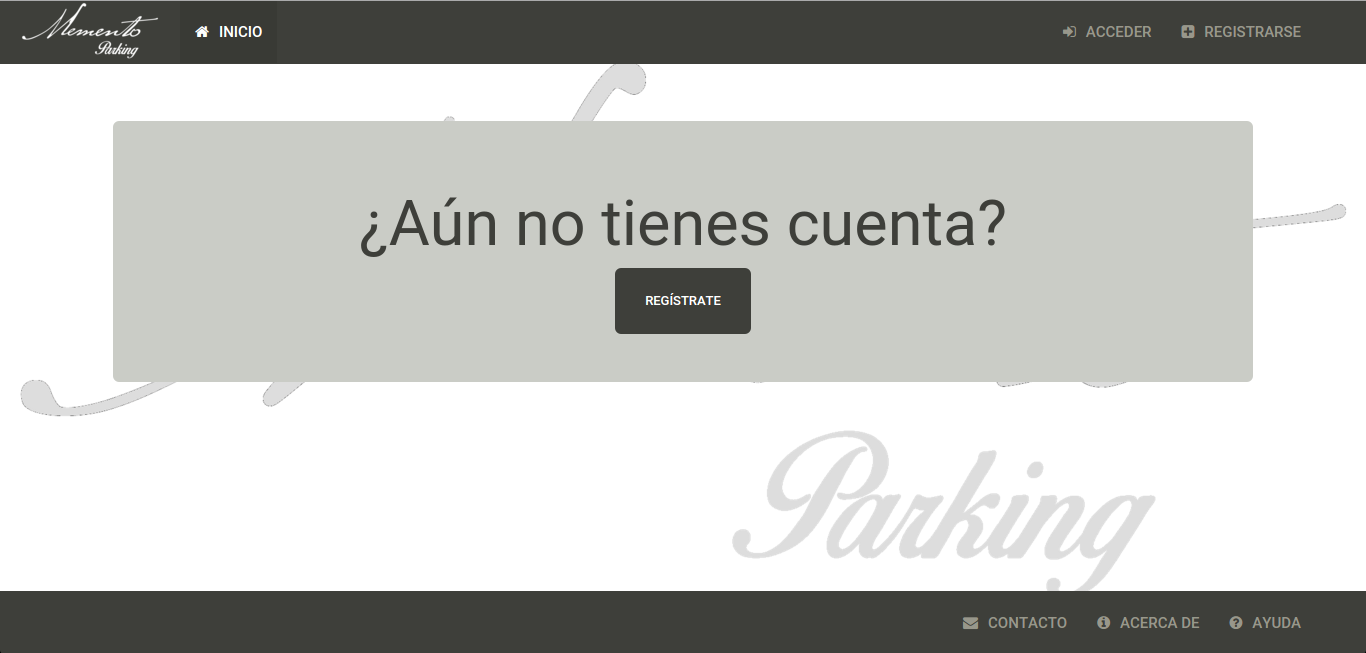
\includegraphics[width=15cm, fbox={\fboxrule} 4mm]{images/05-resultados/04-acceso_usuarios_1.png}
		\caption{Vista previa de la página principal}
		\label{fig:acceso_usuarios_01}
	\end{figure}

	Una vez terminado este paso se comienza con la integración de bootstrap a través de la correspondiente gema y su configuración (ver listado \ref{code:gemfile2}).\\

	\begin{lstlisting}[, frame = single, language = Ruby, caption  = {«Estracto del archivo Gemfile II»}, label = code:gemfile2]
		
		# Use Bootstrap for friendly and responsive UI
		gem 'bootstrap-sass'       # should be already included
		gem 'bootswatch-rails'
		gem 'font-awesome-sass'
		gem 'bootstrap_tokenfield_rails'
		
	\end{lstlisting}
		
	Dotada ya la página de un marco básico de trabajo se procede a extraer los elementos comunes de los enlaces comentados para evitar la repetición de código (premisa básica de Rails DRY -Don't Repeat Yourself-) por lo que se generan una encabezado y pie de página que será común para todo el desarrollo (ver figuras \ref{fig:acceso_usuarios_02} y \ref{fig:acceso_usuarios_03}. Para el diseño adaptado a pantallas de dispositivos móviles ver figuras \ref{fig:acceso_usuarios_04} y \ref{fig:acceso_usuarios_05}). 
	
	\begin{figure}[H]
		\centering
		
\includegraphics[width=15cm, fbox={\fboxrule} 4mm]{images/05-resultados/05-acceso_usuarios_2.png}
		\caption{Vista previa del encabezado}
		\label{fig:acceso_usuarios_02}
	\end{figure}
	
	\begin{figure}[H]
		\centering
		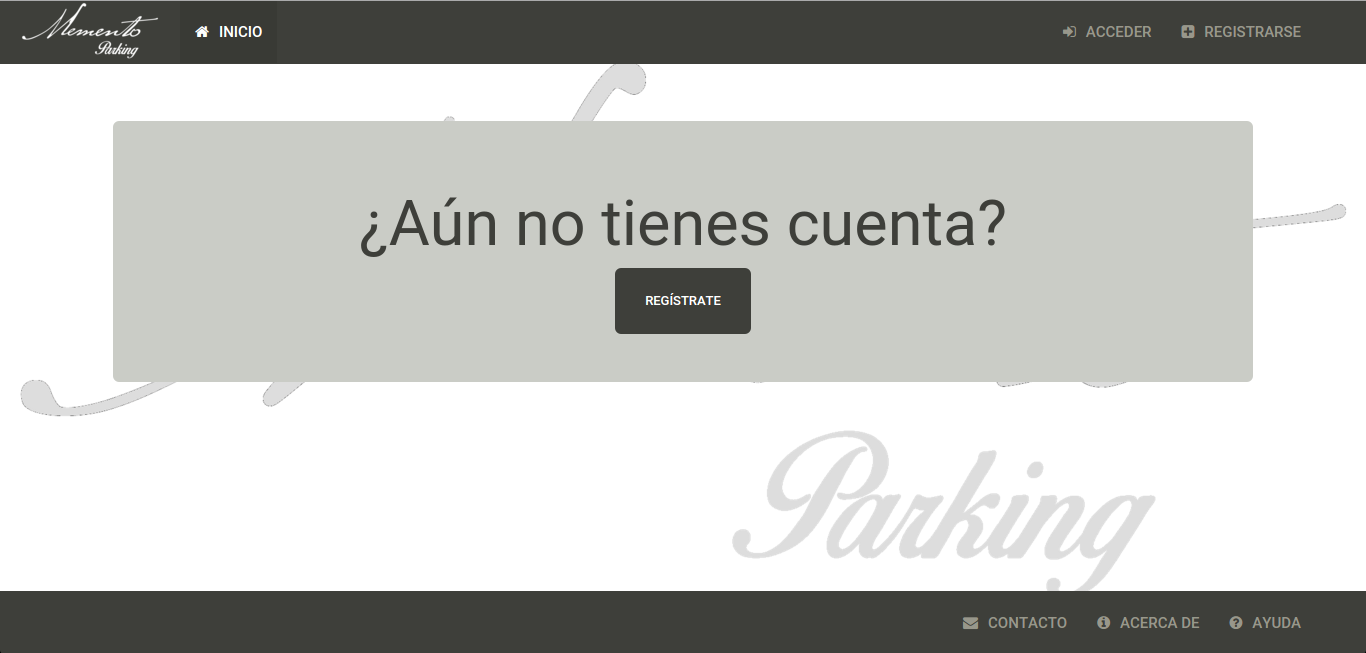
\includegraphics[width=15cm, fbox={\fboxrule} 4mm]{images/05-resultados/06-acceso_usuarios_3.png}
		\caption{Vista previa del pie de página}
		\label{fig:acceso_usuarios_03}
	\end{figure}

	\begin{figure}[H]
		\centering
		
\includegraphics[width=15cm, fbox={\fboxrule} 4mm]{images/05-resultados/07-acceso_usuarios_4.png}
		\caption{Vista previa del encabezado adaptado}
		\label{fig:acceso_usuarios_04}
	\end{figure}
	
		\begin{figure}[H]
		\centering
		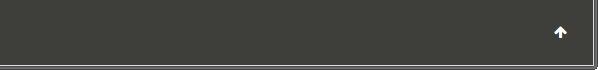
\includegraphics[width=15cm, fbox={\fboxrule} 4mm]{images/05-resultados/08-acceso_usuarios_5.png}
		\caption{Vista previa del pie de página adaptado}
		\label{fig:acceso_usuarios_05}
	\end{figure}
	
	
	A continuación se procede a configurar Devise para permitir el registro de nuevos usuarios, para lo que se creará un nuevo enlace en el encabezado que redirigirá hacia la página de registro que facilita Devise y que será convenientemente modificada (ver figura \ref{fig:acceso_usuarios_06}).
	
	
	\begin{figure}[H]
		\centering
		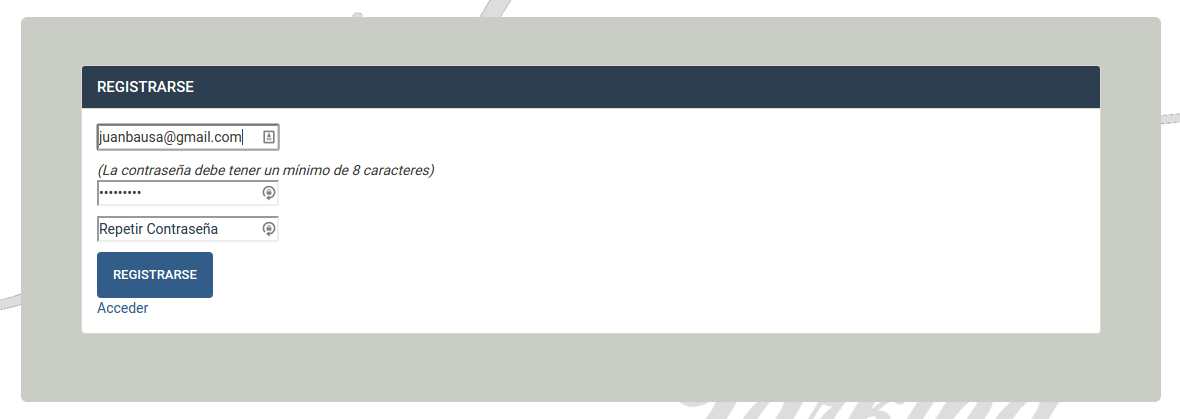
\includegraphics[width=15cm, fbox={\fboxrule} 4mm]{images/05-resultados/09-acceso_usuarios_6.png}
		\caption{Vista previa de la página de registro}
		\label{fig:acceso_usuarios_06}
	\end{figure}
	
	Durante la configuración de Devise resulta necesaria la creación de un modelo para almacenar la información generada (ver listado \ref{code:UserModel}) y la configuración de MongoId para permitir la comunicación con la base de datos creada en MongoLab (ver listado \ref{code:mongoid.yml}).
	
	\begin{lstlisting}[, frame = single, language = Ruby, caption  = {«Archivo de configuración de mongoid»}, label = code:mongoid.yml]
		
		development:
		  clients:
		    default:
		      uri: 'mongodb://<Username>:<Password>@ds061374.mongolab.com:61374/memento_parking'
		      options:
		  options:
		test:
		  clients:
		    default:
		      database: memento_parking_test
		      hosts:
		        - localhost:27017
		      options:
		        read:
		          mode: :primary
		        max_pool_size: 1
		
		production:
		  clients:
		    default:
		      uri: 'mongodb://<Username>:<Password>@ds061374.mongolab.com:61374/memento_parking'
		      options:
		
	\end{lstlisting}
	
	\begin{lstlisting}[, frame = single, language = Ruby, caption  = {«Model User»}, label = code:UserModel]
		
		class User
		  include Mongoid::Document
		  # Include default devise modules. Others available are:
		  # :confirmable, :lockable, :timeoutable and :omniauthable
		  devise :database_authenticatable, :registerable,
		         :recoverable, :rememberable, :timeoutable, :trackable, :validatable, :omniauthable
		
		  ## Database authenticatable
		  field :email,              type: String, default: ''''
		  field :encrypted_password, type: String, default: ''''
		
		  field :name,               type: String
		  field :surname,            type: String
		
		  ## Recoverable
		  field :reset_password_token,   type: String
		  field :reset_password_sent_at, type: Time
		
		  ## Rememberable
		  field :remember_created_at, type: Time
		
		  ## Trackable
		  field :sign_in_count,      type: Integer, default: 0
		  field :current_sign_in_at, type: Time
		  field :last_sign_in_at,    type: Time
		  field :current_sign_in_ip, type: String
		  field :last_sign_in_ip,    type: String
		  
		  embeds_many :car
		end
		
	\end{lstlisting}	
	
	Una vez realizadas estas acciones, se procede a crear un nuevo usuario y comprobar que efectivamente ha sido incorporado a la base de datos (ver figura \ref{fig:acceso_usuarios_07}).
	
	\begin{figure}[H]
		\centering
		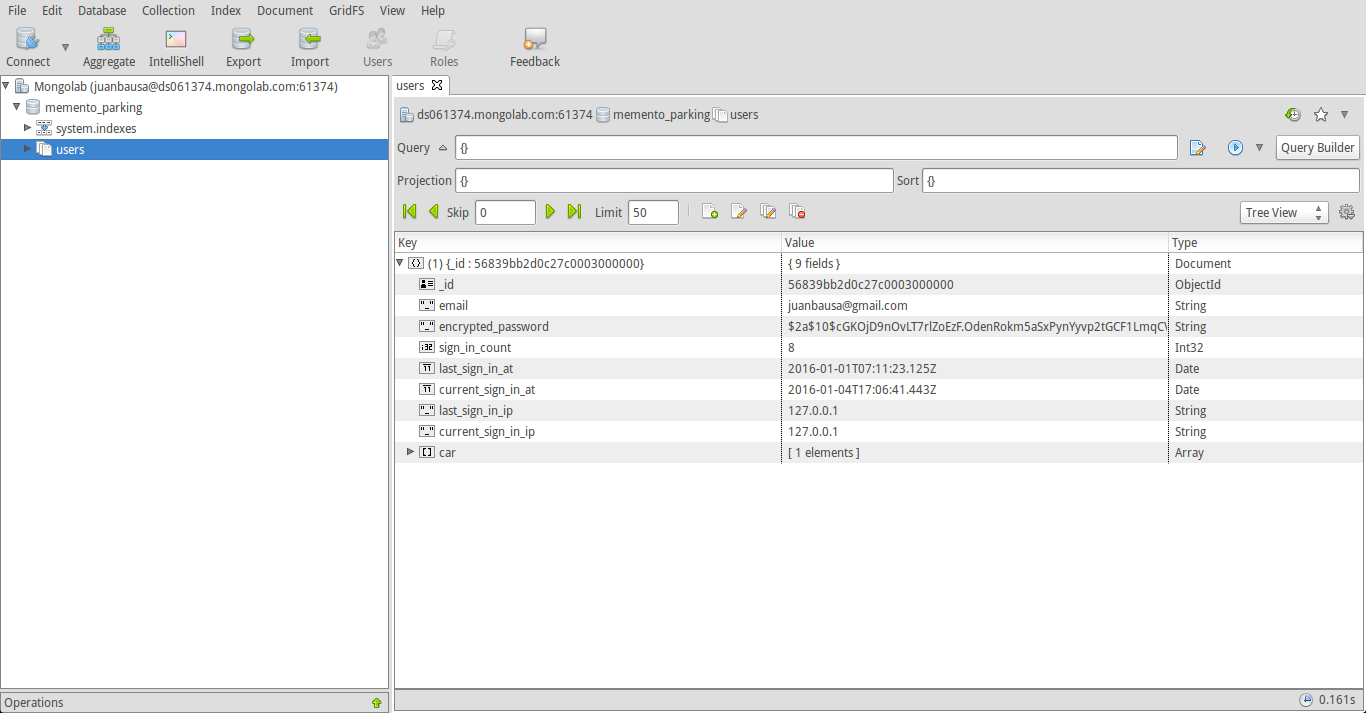
\includegraphics[width=15cm, fbox={\fboxrule} 4mm]{images/05-resultados/10-acceso_usuarios_7.png}
		\caption{Creación nuevo usuario}
		\label{fig:acceso_usuarios_07}
	\end{figure}
	
	\subsubsection{Desarrollo de la Historia de Usuario: ''Acceso de usuarios'' }
	Para el desarrollo de esta historia de usuario es necesario contar con partes del sistema en los que el acceso va a ser restringido para los usuarios anónimos, por lo que el primer paso es crear la página que contendrá el mapa donde se mostrarán las ubicaciones guardadas por el usuario.
	Una vez realizada esta tarea se creará una página para que los usuarios que hayan completado su registro en el sistema puedan acceder al mismo. Ya que devise proporciona una página que se amolda con bastante exactitud a las necesidades del desarrollo, se hace uso de esta vista \textit{mutatis mutandis} (ver figura \ref{fig:acceso_usuarios_08}).
	
	\begin{figure}[H]
		\centering
		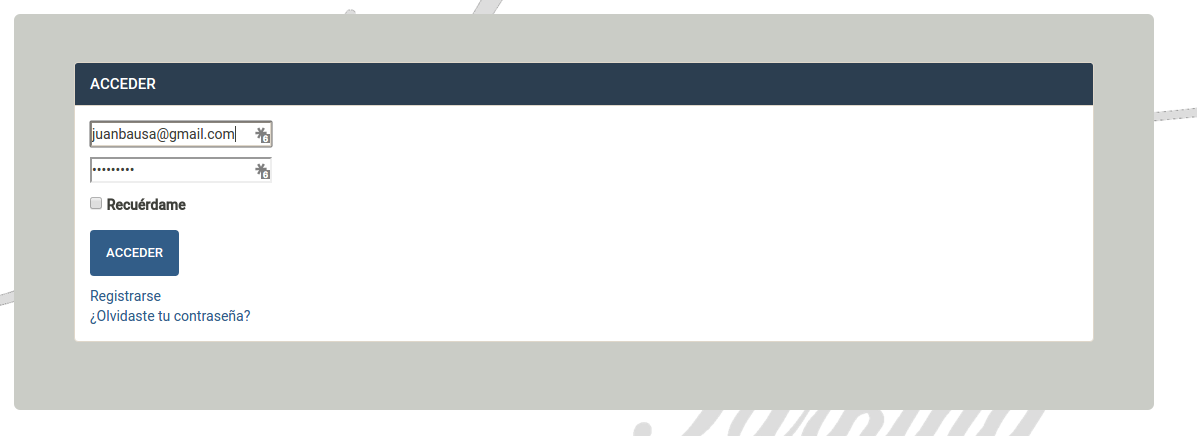
\includegraphics[width=15cm, fbox={\fboxrule} 4mm]{images/05-resultados/11-acceso_usuarios_8.png}
		\caption{Página de acceso a la herrramienta}
		\label{fig:acceso_usuarios_08}
	\end{figure}	
	
	Una vez realizados estos cambios, se procede a configurar devise para restringir el acceso a los usuarios anónimos a las páginas no relativas a la herramienta.
		
	\subsubsection{Desarrollo de la Historia de Usuario: ''Edición de datos de usuarios'' }
	Ya que devise también proporciona una página para la modificación de los datos de usuarios registrados, se procederá a cambiar los campos necesarios para permitir la edición de los datos personales de los usuarios (ver figura \ref{fig:edicion_usuarios}).
	
	\begin{figure}[H]
		\centering
		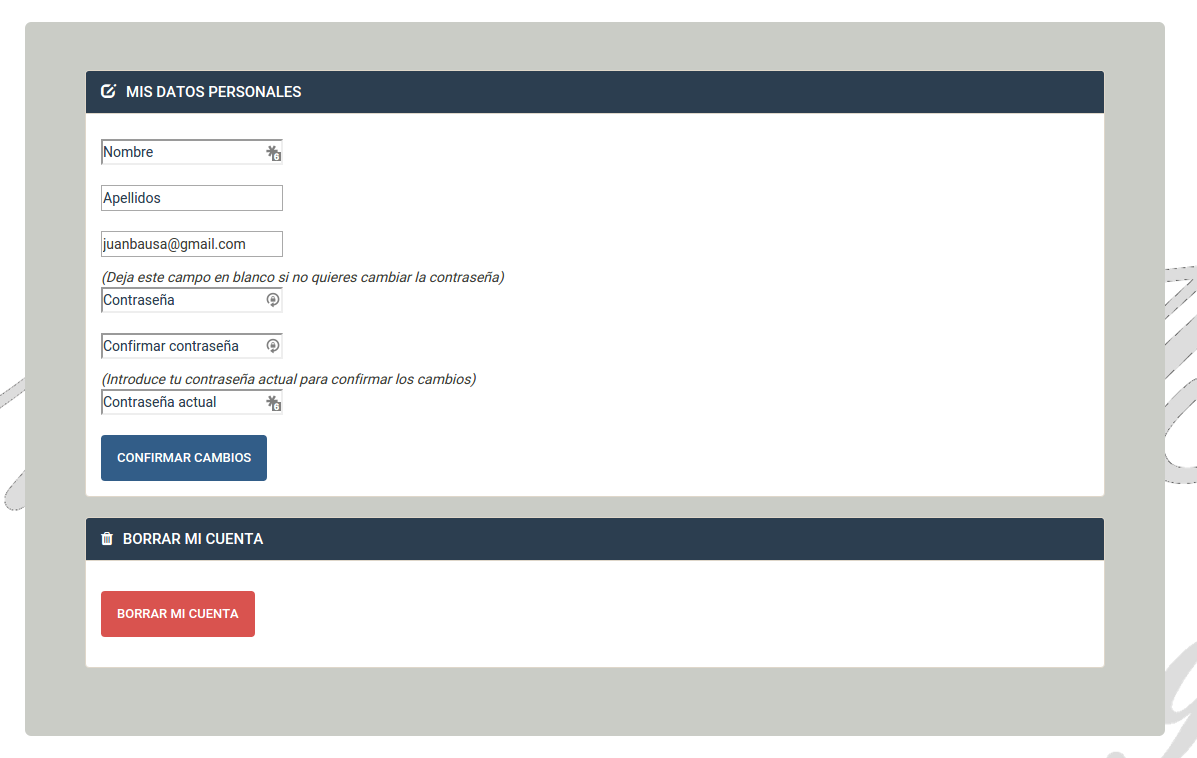
\includegraphics[width=15cm, fbox={\fboxrule} 4mm]{images/05-resultados/12-edicion_usuarios.png}
		\caption{Página de acceso a la herrramienta}
		\label{fig:edicion_usuarios}
	\end{figure}
	
	\subsection{Sprint Review}
	Al término del sprint se ha conseguido una página web de estructura clásica que será el marco de la herramienta, un diseño adaptable a cualquier dispositivo con el que se visite y una gestión básica de usuarios consistente en registro, edición y acceso. También se ha conseguido discriminar a los usuarios anónimos y registrados de manera que el sistema permita o no su acceso a la herramienta. Se crea un primer modelo \textit{User} para la base de datos y se configura gran parte de las herramientas secundarias utilizadas en el desarrollo.

\section{Sprint 2}
En el presente sprint se han llevado a cabo las tareas relacionadas con mostrar al usuario las ubicaciones de sus elementos. Para ello se elige hacerlo en dos formatos, gráficamente a través de un mapa interactivo en el que se mostrarán una serie de marcadores que corresponderán con los elementos del usuario y a través de una serie de cuadros de texto en el que aparecerán las direcciones postales de los elementos del usuario.
	\subsection{Refinamiento del Product Backlog}
	Se realizarán previamente algunas tareas propias de la historia de usuario 7, que se terminará de desarrollar en el sprint 4. Las tareas reubicadas son la creación de un modelo en el esquema de la base de datos para almacenar las ubicaciones geográficas.
	
	\subsection{Planificación de Sprint}
	En este sprint se llevará a cabo la historia de usuario 5. Debido a que se comenzará a trabajar con los mapas interactivos, será necesario acondicionar la página de manera que se pueda incluir este nuevo elemento. La biblioteca elegida para este cometido es la proporcionada por Google, llamada Google Maps, disponible a través de su página web (\href{https://developers.google.com/maps/?hl=es}{API Google Maps}). Esta biblioteca dispone de dos vertientes, la primera es la encargada de mostrar los mapas tal y como se verán por pantalla y la segunda la encargada de la geolocalización directa e inversa, esto es, el intercambio de la información postal a partir de los datos geoespaciales disponibles (latitud y longitud) y el intercambio de de la información geoespacial a partir de los datos postales facilitados, respectivamente. El uso de estas bibliotecas supone la aceptación de los términos y condiciones de uso de Google y la elección de un plan de pago para la utilización. El autor del presente TFG se decantó por el plan gratuito, ya que las limitaciones de uso que se imponen a este plan no afectaran al desarrollo y puesta en marcha inicial del producto. Algunas de estas condiciones son el uso gratuito hasta las 25.000 peticiones de carga de mapas diarias y 2.500 peticiones de resolución de geolocalización diarias. Debido a que el producto no alcanzará el número máximo antes citado, es la opción elegida.\\
	Puesto que en este momento del desarrollo los usuarios aún no pueden almacenar las ubicaciones, se editará la base de datos manualmente para incluir los datos necesarios para poder mostrar elementos en el mapa del usuario. Para almacenar en la base de datos los elementos que incluirán los datos geoespaciales, se procederá a crear un nuevo modelo de datos llamado ''Cars''. Este nuevo modelo quedará embebido dentro del documento ''User''. Esta decisión de diseño corresponde al incremento de velocidad en las búsquedas que se logra al incorporar el modelo ''Cars'' al modelo ''Users'' y que se considera que el número de documentos de este tipo que se incorporarán no pondrá en peligro la integridad del esquema.\\
	La pila de sprint es la siguiente:\\

	\begin{table}[H]
	  \centering 
	 	\begin{tabular}{p{0.4\linewidth}p{0.4\linewidth}}
	    \toprule
	    \multicolumn{2}{c}{\cellcolor{black!30}\textbf{Historia de Usuario}} 													\\
		\multicolumn{2}{l}{\cellcolor{gray!25}\textbf{Número: }5}																\\
		\multicolumn{2}{l}{\textbf{Nombre Historia: } Mostrar posiciones geoespaciales y direcciones postales}				\\
		\cellcolor{gray!25}\textbf{Valor de negocio: Alto}	&	\cellcolor{gray!25}\textbf{Riesgo en desarrollo: Medio}		\\
		\textbf{Esfuerzo:} 12 horas				&	\textbf{Sprint asignado: }2 												\\
		\multicolumn{2}{l}{\cellcolor{gray!25}\textbf{Programador responsable: }Juan Bausá}									\\
		\multicolumn{2}{l}{\textbf{Descripción:}}                                                     						\\
		\multicolumn{2}{l}{\parbox{15cm}{Mostrar los datos de localización geoespacial en un mapa mediante la inclusión de elementos visuales adecuados a la representación. Mostrar los datos de localización postal en un elemento de texto adecuado.}}				\\
		\multicolumn{2}{l}{\cellcolor{gray!25}\textbf{Resultado:}}																\\		
		\multicolumn{2}{l}{\parbox{15cm}{Los usuarios registrados podrán ver la ubicación de los elementos almacenados tanto en un mapa como en un cuadro de texto.}}																									\\
		\multicolumn{2}{l}{\textbf{Tareas:}}																					\\
		\multicolumn{2}{l}{
			\begin{minipage}{12cm}
	    		\vskip 4pt
	    		\begin{itemize}
	    			\item Crear una nueva página contenedora ''map'' para la nueva funcionalidad
	    			\item Creación de un nuevo modelo ''Cars'' para almacenar los datos relativos a los elementos geoespaciales.
	    			\item Edición de la base de datos para almacenar datos de nuevos elementos con posición geográfica controlada.
	    			\item Creación de un elemento contenedor para mostrar el mapa.
	    			\item Llamada a la API proporcionada por Google para mostrar el mapa.
	    			\item Centrar mapa a la posición del usuario.
	    			\item Llamada a la API proporcionada por Google para lograr la localización geoespacial y postal de los elementos.
	    			\item Tratamiento de los datos devueltos por la API proporcionada por Google para mostrarlos de manera adecuada y entendible por el usuario.
				\end{itemize}
			  	\vskip 4pt
		 	\end{minipage}
		} \\																				
	    \hline
	  \end{tabular}
	  \caption{Historia de Usuario 5}
	\end{table}
		
	\subsubsection{Desarrollo de la Historia de Usuario: ''Mostrar posiciones geoespaciales y direcciones postales''}
	Como se ha comentado en apartado anterior, para la realización de esta historia de usuario se comienza añadiendo un nuevo modelo de datos llamado ''Car'' (ver listado \ref{code:CarModel}) y editando manualmente la base de datos a través de MongoChef para incluir los datos relativos al documento ''car'' (ver listado \ref{code:mostrar_posiciones}) para un usuario existente. Se incorporan unos datos geoespaciales y postales controlados por el desarrollador como datos válidos.
	
	\begin{lstlisting}[, frame = single, language = Ruby, caption  = {«Model Car»}, label = code:CarModel]
		
		class Car
		  include Mongoid::Document
		  embedded_in :user
		  field :coordinates, type: String
		  field :description, type: String
		  field :address, type: String
		end
		
	\end{lstlisting}

	\begin{lstlisting}[, frame = single, language = JSON, caption  = {«Documento JSON relativo a un elemento \textit{coche}»}, label = code:mostrar_posiciones]
		
		{ 
		    "_id" : ObjectId("56839bb2d0c27c0003000000"), 
		    "email" : "juanbausa@gmail.com", 
		    "encrypted_password" : "$2a$10$cGKOjD9nOvLT7rlZoEzF.OdenRokm5aSxPynYyvp2tGCF1LmqCVtm", 
		    "sign_in_count" : NumberInt(12), 
		    "last_sign_in_at" : ISODate("2016-01-08T16:55:26.390+0000"), 
		    "current_sign_in_at" : ISODate("2016-01-08T18:33:10.662+0000"), 
		    "last_sign_in_ip" : "127.0.0.1", 
		    "current_sign_in_ip" : "127.0.0.1", 
		    "car" : [
		        {
		            "_id" : ObjectId("56839de073e3e125cd000000"), 
		            "description" : "TOYOTITA", 
		            "coordinates" : "(38.993038383938284, -3.921668529510498)", 
		            "address" : "Calle Carlos López Bustos, 1, 13005 Ciudad Real, Cdad. Real, España", 
		            "shared" : [
		                "janedoe@gmail.com", 
		                "johndoe@gmail.com"
		            ]
		        }
		    ]
		}
		
	\end{lstlisting}
	
	A continuación, y una vez dado de alta en la API proporcionada por Google y generadas las claves necesarias para su utilización, se crea un elemento HTML que contendrá el mapa generado y se hace una llamada al API de manera que se muestre el mapa donde se generarán los elementos de marcado (ver figura \ref{fig:mostrar_posiciones2}).\\

	\begin{figure}[H]
		\centering
		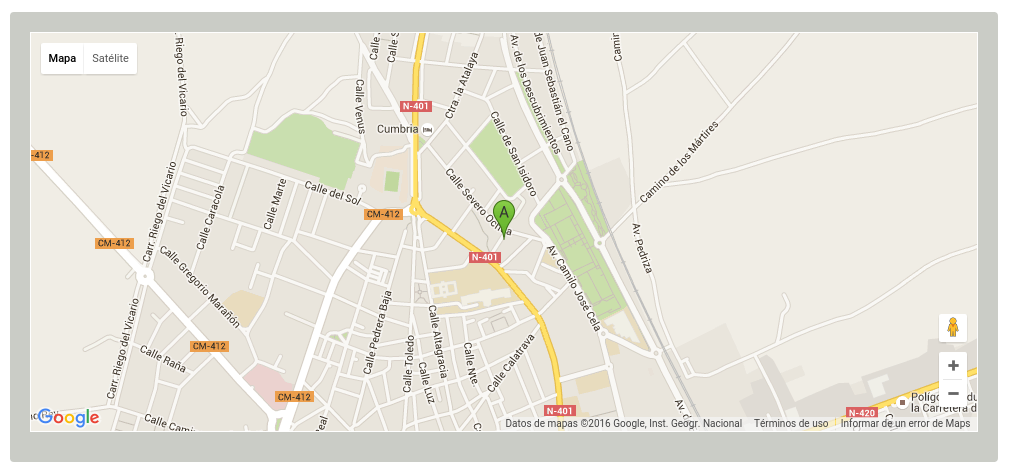
\includegraphics[width=15cm, fbox={\fboxrule} 4mm]{images/05-resultados/14-mostrar_posiciones_2.png}
		\caption{Elementos \textit{coche} y dirección postal almacenada}
		\label{fig:mostrar_posiciones2}
	\end{figure}
	
	 Para el centrado del mapa en la posición del usuario se utiliza la propiedad proporcionada por HTML5 para conocer la ubicación geográfica aproximada del usuario y se modifican las propiedades del mapa para centrarlo en la posición adquirida (ver listado \ref{code:geocodeHTML5}).
	 
	 	\begin{lstlisting}[, frame = single, language = JavaScript, caption  = {«Geolocalización HTML5»}, label = code:geocodeHTML5]
		
		function getLocation() {
 		if (navigator.geolocation) {
 			coords = null;
 			navigator.geolocation.getCurrentPosition(set_map_Location);
 		}
 	}
		
	\end{lstlisting}
	 
	Con el mapa centrado en la posición del usuario se realiza una llamada a la base de datos para recuperar los elementos previamente guardados y mediante un bucle se crean dinámicamente los elementos HTML que mostrarán los datos postales  y se hace una llamada a una función JavaScript que será la encargada de utilizar el API de Google Maps para incorporar marcadores en las coordenadas geoespaciales recuperadas de la base de datos (ver listado \ref{code:markerDB}), al término de la tarea, se modifican los elementos HTML para que incorporen los datos postales de los marcadores.
	
		\begin{lstlisting}[, frame = single, language = JavaScript, caption  = {«Añadir marcadores desde base de datos»}, label = code:markerDB]
	/* Add markers stored in DB */
	 function addMarkerDB(address, description) {

	 	if (markerUserClick) {
	 		markerUserClick.setMap(null);
	 		markerUserClick = null;
	 	}

	 	if(address){
	 		geocoder.geocode({'address': address}, function(results, status) {
	 			if (status === google.maps.GeocoderStatus.OK) {
	 				var markerDB = new google.maps.Marker({
	 					map: map,
	 					draggable: true,
	 					position: results[0].geometry.location
	 				});
	 				var infoWindowDB = new google.maps.InfoWindow({size: new google.maps.Size(150,50)});
	 				infoWindowDB.setContent(''<b>''+description+'':</b><br>''+ results[0].formatted_address);
	 				setMarkerDB(markerDB);
	 				google.maps.event.addListener(markerDB, 'click', function(){infoWindowDB.open(map,markerDB);});
	 			} else {
	 				alert('Geocode was not successful for the following reason: ' + status);
	 			}
	 		});
	 	}
	 }
	 \end{lstlisting}
	
	\subsection{Sprint Review}
	Al término de este sprint se ha logrado que el usuario registrado pueda ver un mapa interactivo en el que se muestran marcadores correspondientes a los elementos almacenados en la base de datos. De igual manera, se crean tantos elementos contenedores como ubicaciones estuvieran guardadas y se rellenan con los datos postales correspondientes. El usuario podrá ver de esta manera de forma entendible a través del mapa y los cuadros de texto la ubicación de los elementos almacenados. Ha sido necesario reubicar algunas tareas previstas en la historia de usuario 7 en el sprint 4 como condición previa para llevar a término este sprint.
	
\section{Sprint 3}
En el presente sprint se llevarán a cabo las tareas relacionadas con el almacenaje de las coordenadas geoespaciales y postales de los elementos del usuario. El objetivo completo se logrará en el sprint 5 con la consecución de la historia de usuario 6, ya que en esta primera aproximación el usuario tendrá a su disposición únicamente un elemento sobre el que guardar posiciones geográficas.

	\subsection{Refinamiento del Product Backlog}
	No se modifica el \textit{Product Backlog}.
	
	\subsection{Planificación de Sprint}
	En este sprint se desarrollará la historia de usuario 4, que consiste en permitir al usuario almacenar ubicaciones geográficas usando para ello elementos predeterminados denominados \textit{coches}. 
	%Lograr este objetivo requiere que el usuario pueda seleccionar previamente entre sus \textit{coches} aquel que va a modificar su ubicación. La selección de la nueva ubicación se hará pulsando sobre el mapa y confirmando la operación mediante un botón creado al efecto. 
	La confirmación para disparar la acción de almacenaje en la base de datos correrá a cargo de un botón creado al efecto.
	Una vez realizada la operación se informará al usuario de la correcta o errónea finalización de la misma haciendo uso de los mensajes de respuesta que Rails pone a disposición del desarrollador a través del \textit{helper} correspondiente.
	
	\begin{table}[H]
	  \centering 
	 	\begin{tabular}{p{0.4\linewidth}p{0.4\linewidth}}
	    \toprule
	    \multicolumn{2}{c}{\cellcolor{black!30}\textbf{Historia de Usuario}} 													\\
		\multicolumn{2}{l}{\cellcolor{gray!25}\textbf{Número: }4}																\\
		\multicolumn{2}{l}{\textbf{Nombre Historia: } Guardar posiciones geoespaciales y direcciones postales}				\\
		\cellcolor{gray!25}\textbf{Valor de negocio: Alto}	&	\cellcolor{gray!25}\textbf{Riesgo en desarrollo: Medio}		\\
		\textbf{Esfuerzo:} 30 horas				&	\textbf{Sprint asignado: }3 												\\
		\multicolumn{2}{l}{\cellcolor{gray!25}\textbf{Programador responsable: }Juan Bausá}									\\
		\multicolumn{2}{l}{\textbf{Descripción:}}                                                     						\\
		\multicolumn{2}{l}{\parbox{15cm}{Guardar los datos de localización geoespacial seleccionados en el mapa mediante la interacción del usuario.}}				\\
		\multicolumn{2}{l}{\cellcolor{gray!25}\textbf{Resultado:}}																\\		
		\multicolumn{2}{l}{\parbox{15cm}{Los usuarios registrados podrán modificar la ubicación del elemento \textit{coche} haciendo uso del mapa interactivo.}}																									\\
		\multicolumn{2}{l}{\textbf{Tareas:}}																					\\
		\multicolumn{2}{l}{
			\begin{minipage}{12cm}
	    		\vskip 4pt
	    		\begin{itemize}
	    			\item Recuperar la ubicación geoespacial y postal de la posición seleccionada en el mapa por el usuario mediante pulsación del ratón.
	    			\item Guardar la ubicación en la base de datos al pulsar en el botón correspondiente creado al efecto en la página.
	    			\item Informar al usuario de la correcta realización de la operación o mostrar un mensaje de error en caso contrario.
	    			\item Modificación de los mensajes de error, aviso e información por defecto del sistema para hacerlos visualmente homogéneos al resto de la página.
				\end{itemize}
			  	\vskip 4pt
		 	\end{minipage}
		} \\																				
	    \hline
	  \end{tabular}
	  \caption{Historia de Usuario 4}
	\end{table}
	
	\subsubsection{Desarrollo de la Historia de Usuario: ''Guardar ubicaciones geoespaciales y postales''}
	
	Gracias a la API de Google Maps, se puede recuperar fácilmente la ubicación geoespacial de la posición donde se detecta un evento de pulsación sobre el mapa (ver listado \ref{code:clickMarker}) y puede mostrarse en un bloque de texto la información postal recuperada, de forma que el usuario tenga un conocimiento completo de cual es la ubicación seleccionada (ver figura \ref{fig:guardar_posiciones_1}).
	
	\begin{lstlisting}[language = JavaScript, frame = lines, caption  = {«Añadir marcador al mapa cuando el usuario pulsa con el ratón»}, label = code:clickMarker]
	
	 // A function to create the marker and set up the event window function 
	 function createMarkerLatLng(latlng) {
	 	markerUserClick = new google.maps.Marker(
	 		{position: latlng, 
	 			icon: ''https://mt.google.com/vt/icon?psize=20&font=fonts/Roboto-Regular.ttf&color=ff330000&name=icons/spotlight/spotlight-waypoint-blue.png'',
	 			map: map, 
	 			zIndex: Math.round(latlng.lat()*-100000)<<5}
	 			);
	 	geocoder.geocode({'location': latlng}, function(results, status) {
	 		if (status === google.maps.GeocoderStatus.OK) {
	 			if (results[0]) {
	 				map.setZoom(15);
	 				address = results[0].formatted_address;
	 				infowindow.setContent(''<b>Nueva ubicación:</b><br>'' + results[0].formatted_address);
	 				infowindow.open(map, markerUserClick);
	 			} else {
	 				window.alert('No results found');
	 			}
	 		} else {
	 			window.alert('Geocoder failed due to: ' + status);
	 		}
	 	});
	 	google.maps.event.trigger(markerUserClick, 'click');
	 }
	 
	 \end{lstlisting}

	\begin{figure}[H]
		\centering
		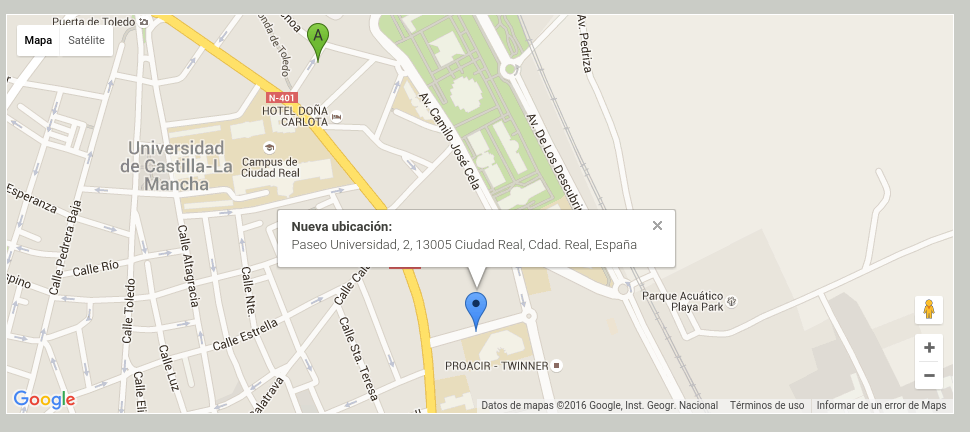
\includegraphics[width=15cm, fbox={\fboxrule} 4mm]{images/05-resultados/15-guardar_posiciones_1.png}
		\caption{Marcador personalizado con información de dirección postal}
		\label{fig:guardar_posiciones_1}
	\end{figure}
	 
	El almacenamiento de la ubicación se hará mediante una llamada a una dirección concreta con los parámetros necesarios para que el controlador correspondiente llame a la base de datos para completar la operación (ver listado \ref{code:coordsController}). 
	
	\begin{lstlisting}[, frame = single, language = Ruby, caption  = {«Guardar coordenadas»}, label = code:coordsController]
	  def coords
	      @user = User.find_by(email: params[:mailOwner])
	      @car = @user.car.find(params[:carId])
	
	    if @car.update({coordinates: params[:coord], address: params[:address]})
	      flash[:success] = ''Dirección actualizada correctamente''
	    else
	      flash[:alert] = ''Error al actualizar la dirección''
	    end
	    redirect_to maps_path
	  end
	\end{lstlisting}
	
	Una vez realizado esto, se informa al usuario mediante un mensaje de la resolución correcta o incorrecta del mismo. Rails brinda un \textit{helper} que facilita la retroalimentación de este tipo, pero se limita a mensajes de texto plano, lo que rompe con la visualización de la página, por lo que se modifica mediante código para conseguir un aspecto homogéneo mediante bootstrap a estos mensajes (ver figura \ref{fig:guardar_posiciones_2} y listado \ref{code:flashMessages}).
	
	\begin{figure}[H]
		\centering
		
\includegraphics[width=15cm, fbox={\fboxrule} 4mm]{images/05-resultados/16-guardar_posiciones_2.png}
		\caption{Mensaje reenviado por el controlador}
		\label{fig:guardar_posiciones_2}
	\end{figure}
		
	\begin{lstlisting}[frame = single, language = Ruby, caption  = {«Código para sobreescribir los mensajes flash»}, label = code:flashMessages]
		# https://gist.github.com/suryart/7418454
		module ApplicationHelper
		  def bootstrap_class_for flash_type
		    { success: "alert-success", error: "alert-error", alert: "alert-warning", notice: "alert-info" }[flash_type.to_sym] || flash_type.to_s
		end
		
		  def flash_messages(opts = {})
		    #flash.except(:timedout).each do |msg_type, message|
		    flash.each do |msg_type, message|
		      if message != true
		        concat(content_tag(:div, message, class: "alert #{bootstrap_class_for(msg_type)} fade in", style: "margin-top:10px;") do 
		                concat content_tag(:button, 'x', class: "close", data: { dismiss: 'alert' })
		                concat message 
		              end)
		      end
		    end
		    nil
		  end
		end
	\end{lstlisting}	
		
	\subsection{Sprint Review}
	Al término de este sprint se ha conseguido que el usuario pueda seleccionar ubicaciones geográficas mediante pulsaciones de ratón sobre el mapa e informarle de cual es la dirección postal seleccionada mediante su inclusión en cuadros de texto creados al efecto. La confirmación del almacenamiento de la nueva ubicación se ha realizado mediante un botón que dispara la acción. La retroalimentación al usuario se ha conseguido mediante la inclusión de mensajes informativos del estado de la acción. 

\section{Sprint 4}
	En el presente sprint se realizarán las tareas necesarias para que el usuario pueda crear nuevos elementos sobre los que almacenar ubicaciones.
	
	\subsection{Refinamiento del Product Backlog}
	No se realiza ninguna modificación del \textit{Product Backlog}.
	
	\subsection{Planificación de Sprint}
	En este sprint se desarrollará la historia de usuario 7, consistente en que el usuario pueda generar nuevos elementos sobre los que almacenar posiciones geográficas. Las tareas a llevar a cabo son similares a las implementadas en la historia de usuario 3 durante el sprint 1, puesto que consiste en la creación de elementos de la base de datos. Las diferencias detectadas vienen definidas por el esquema de la base de datos, puesto que en este momento se modificará un documento embebido en lugar del documento principal.
	
	\begin{table}[H]
	  \centering 
	 	\begin{tabular}{p{0.4\linewidth}p{0.4\linewidth}}
	    \toprule
	    \multicolumn{2}{c}{\cellcolor{black!30}\textbf{Historia de Usuario}} 													\\
		\multicolumn{2}{l}{\cellcolor{gray!25}\textbf{Número: }7}																\\
		\multicolumn{2}{l}{\textbf{Nombre Historia: } Crear nuevos elementos \textit{coche}}				\\
		\cellcolor{gray!25}\textbf{Valor de negocio: Alto}	&	\cellcolor{gray!25}\textbf{Riesgo en desarrollo: Medio}		\\
		\textbf{Esfuerzo:} 12 horas				&	\textbf{Sprint asignado: }4												\\
		\multicolumn{2}{l}{\cellcolor{gray!25}\textbf{Programador responsable: }Juan Bausá}									\\
		\multicolumn{2}{l}{\textbf{Descripción:}}                                                     						\\
		\multicolumn{2}{l}{\parbox{15cm}{Crear y editar nuevos elementos \textit{coche} que permitan almacenar nuevas ubicaciones geoespaciales.}}				\\
		\multicolumn{2}{l}{\cellcolor{gray!25}\textbf{Resultado:}}																\\		
		\multicolumn{2}{l}{\parbox{15cm}{Los usuarios registrados podrán crear nuevos elementos \textit{coche} donde podrán almacenar ubicaciones geográficas haciendo uso de las herramientas implementadas en el anterior sprint.}}																	\\
		\multicolumn{2}{l}{\textbf{Tareas:}}																					\\
		\multicolumn{2}{l}{
			\begin{minipage}{12cm}
	    		\vskip 4pt
	    		\begin{itemize}
	    			\item Crear una nueva página contenedora ''car'' para la nueva funcionalidad
	    			\item Añadir un método de selección que permita crear un nuevo elemento
	    			\item Añadir un botón de confirmación de los cambios
	    			\item Añadir mensajes de confirmación o error resultantes de llevar a cabo la acción
				\end{itemize}
			  	\vskip 4pt
		 	\end{minipage}
		} \\																				
	    \hline
	  \end{tabular}
	  \caption{Historia de Usuario 7}
	\end{table}
	
	\subsubsection{Desarrollo de la Historia de Usuario: ''Creación de elementos \textit{coche}''}
	Se crea una nueva página contenedora para la funcionalidad (ver figura \ref{fig:crear_coche}). Debido a que ya se realizaron ciertas tareas concernientes a la historia de usuario que se está desarrollando, no es necesario modificar el esquema de la base de datos. Se añade un elemento que permite crear un nuevo elemento.
	
	\begin{figure}[H]
		\centering
		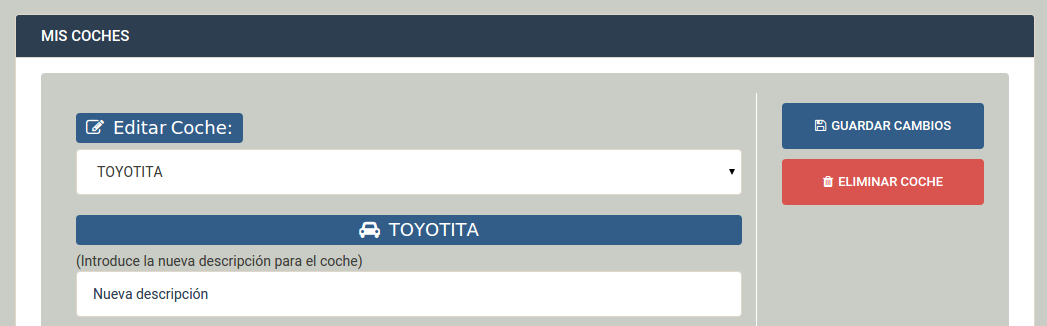
\includegraphics[width=15cm, fbox={\fboxrule} 4mm]{images/05-resultados/17-crear_coche.png}
		\caption{Página de edición de elementos \textit{coche}}
		\label{fig:crear_coche}
	\end{figure}	
	
	Al hacer efectiva la selección aparece un formulario hasta el momento oculto que permite la creación del elemento indicando el nombre con el que se visualizará.
	La confirmación de los cambios se realiza mediante un botón que dispara la acción del controlador, encargado final de comunicar a la base de datos los cambios a realizar (ver listado \ref{code:newCar}).
	
	\begin{lstlisting}[, frame = single, language = Ruby, caption  = {«Creación elemento \textit{coche}»}, label = code:newCar]
		def newCar
		    mail = current_user.email
		    @user = User.find_by(email: mail)    
		    if params[:newdescription] != ''''
		      @user.car.create!(description: params[:newdescription])
		      flash[:success] = ''Se ha creado un nuevo coche''
		    else
		      flash[:alert] = ''Error al crear el nuevo coche. Introduce una descripción.''
		    end
		    redirect_to car_path
		  end	
	\end{lstlisting}
	
	Con la respuesta de la base de datos se envía un mensaje al usuario informando de la terminación correcta o errónea de la acción (ver figura \ref{fig:crear_coche2}).
		
	\begin{figure}[H]
		\centering
		
\includegraphics[width=15cm, fbox={\fboxrule} 4mm]{images/05-resultados/18-crear_coche2.png}
		\caption{Respuesta controlador al crear nuevo coche}
		\label{fig:crear_coche2}
	\end{figure}
		
	\subsection{Sprint Review}
	Al término de este sprint se consigue que el usuario pueda crear nuevos elementos sobre los que almacenar ubicaciones.

\section{Sprint 5}
	En el presente sprint se llevarán a cabo las tareas necesarias para que el usuario pueda seleccionar sobre que elemento \textit{coche} desea almacenar la ubicación seleccionada en el mapa.
	\subsection{Refinamiento del Product Backlog}
	No se producen cambios en el \textit{Product Backlog}.
	
	\subsection{Planificación de Sprint}
	En este sprint se desarrollará la historia de usuario 6, consistente en permitir al usuario seleccionar sobre que elemento \textit{coche} quiere llevar a cabo la tarea de almacenaje de ubicación. La selección se realizará mediante la inclusión de elementos representativos de los \textit{coches} que el usuario tiene almacenados en la base de datos.
	
	\begin{table}[H]
	  \centering 
	 	\begin{tabular}{p{0.4\linewidth}p{0.4\linewidth}}
	    \toprule
	    \multicolumn{2}{c}{\cellcolor{black!30}\textbf{Historia de Usuario}} 													\\
		\multicolumn{2}{l}{\cellcolor{gray!25}\textbf{Número: }6}																\\
		\multicolumn{2}{l}{\textbf{Nombre Historia: } Seleccionar un elemento y mostrarlo en el mapa}							\\
		\cellcolor{gray!25}\textbf{Valor de negocio: Alto}	&	\cellcolor{gray!25}\textbf{Riesgo en desarrollo: Bajo}		\\
		\textbf{Esfuerzo:} 10 horas				&	\textbf{Sprint asignado: }5 												\\
		\multicolumn{2}{l}{\cellcolor{gray!25}\textbf{Programador responsable: }Juan Bausá}									\\
		\multicolumn{2}{l}{\textbf{Descripción:}}                                                     						\\
		\multicolumn{2}{l}{\parbox{15cm}{Seleccionar uno de los elementos disponibles y mostrarlo en el mapa.}}				\\
		\multicolumn{2}{l}{\cellcolor{gray!25}\textbf{Resultado:}}																\\		
		\multicolumn{2}{l}{\parbox{15cm}{Los usuarios podrán seleccionar un elemento de la lista disponible y se mostrará su ubicación en el mapa mediante un marcador.}}																									\\
		\multicolumn{2}{l}{\textbf{Tareas:}}																					\\
		\multicolumn{2}{l}{
			\begin{minipage}{12cm}
	    		\vskip 4pt
	    		\begin{itemize}
	    			\item Modificar la lista de elementos para mostrar al usuario la sensación de \textit{pulsado}.
	    			\item Limpiar el mapa de todos los marcadores de los elementos excepto el seleccionado y la posición del usuario.
				\end{itemize}
			  	\vskip 4pt
		 	\end{minipage}
		} \\																				
	    \hline
	  \end{tabular}
	  \caption{Historia de Usuario 6}
	\end{table}
	
	\subsubsection{Desarrollo de la Historia de Usuario: ''Seleccionar y mostrar un elemento en el mapa''}
	Para la selección de los elementos se decide crear una lista con todos los marcadores existentes en la base de datos del usuario y modificar sus propiedades para que al detectar una pulsación, la configuración de colores cambie(ver figura \ref{fig:seleccionar_coche}), de manera que el usuario visualice rápidamente si existe algún elemento seleccionado y en caso afirmativo cual es. \\
	
	\begin{figure}[H]
		\centering
		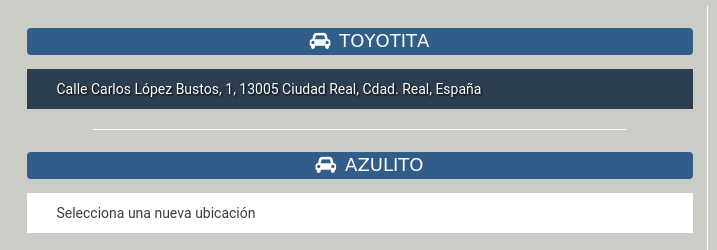
\includegraphics[width=15cm, fbox={\fboxrule} 4mm]{images/05-resultados/19-seleccionar_coche.png}
		\caption{Selector de elementos \textit{coche}}
		\label{fig:seleccionar_coche}
	\end{figure}	
		
	Al seleccionar un elemento de la lista, la página se reposiciona para que el foco vuelva al mapa y se redibuja el mapa dejando únicamente los marcadores pertenecientes a la ubicación actual del usuario y de la ubicación del elemento seleccionado, logrando de esta manera una funcionalidad secundaria que podría traducirse por ''Quiero ver un solo marcador de elemento en el mapa''.\\
			
	\subsection{Sprint Review}
	Al término de este sprint se ha logrado que el usuario puede elegir sobre cual de los elementos \textit{coche} creados en el anterior sprint desea almacenar la ubicación geográfica, dando la posibilidad de mantener tantos \textit{coches} como se desee.

\section{Sprint 6}
	En este sprint se llevará a cabo el desarrollo de la historia de usuario 8, consistente en permitir la edición de las propiedades de los elementos \textit{coche}. De igual manera se permite la eliminación de elementos \textit{coche}.
	\subsection{Refinamiento del Product Backlog}
	No se modifica el \textit{Product Backlog}.
	
	\subsection{Planificación de Sprint}
	En este sprint se desarrollará la historia de usuario 8, que consiste en permitir al usuario modificar las propiedades del elemento \textit{coche}. Es una ampliación de la historia de usuario 7 desarrollada en el sprint 4, puesto que ya se ha desarrollado una página donde poder llevar a cabo estas tareas y una forma de selección del elemento a modificar o eliminar. La edición de las propiedades, la modificación o eliminación en la base de datos y la respuesta al usuario en forma de mensaje es similar a lo llevado a cabo en el sprint 1 y 4 con la edición de los datos del propio usuario y la creación de nuevos elementos \textit{coche}.
	
	\begin{table}[H]
	  \centering 
	 	\begin{tabular}{p{0.4\linewidth}p{0.4\linewidth}}
	    \toprule
	    \multicolumn{2}{c}{\cellcolor{black!30}\textbf{Historia de Usuario}} 													\\
		\multicolumn{2}{l}{\cellcolor{gray!25}\textbf{Número: }8}																\\
		\multicolumn{2}{l}{\textbf{Nombre Historia: } Seleccionar un elemento \textit{coche} y modificar sus propiedades}							\\
		\cellcolor{gray!25}\textbf{Valor de negocio: Medio}	&	\cellcolor{gray!25}\textbf{Riesgo en desarrollo: Bajo}		\\
		\textbf{Esfuerzo:} 12 horas				&	\textbf{Sprint asignado: }6 												\\
		\multicolumn{2}{l}{\cellcolor{gray!25}\textbf{Programador responsable: }Juan Bausá}									\\
		\multicolumn{2}{l}{\textbf{Descripción:}}                                                     						\\
		\multicolumn{2}{l}{\parbox{15cm}{Seleccionar uno de los elementos \textit{coche} y modificar sus propiedades.}}				\\
		\multicolumn{2}{l}{\cellcolor{gray!25}\textbf{Resultado:}}																\\		
		\multicolumn{2}{l}{\parbox{15cm}{Los usuarios podrán seleccionar un elemento \textit{coche} y modificar sus propiedades.}}																								\\
		\multicolumn{2}{l}{\textbf{Tareas:}}																					\\
		\multicolumn{2}{l}{
			\begin{minipage}{12cm}
	    		\vskip 4pt
	    		\begin{itemize}
	    			\item Crear un botón para eliminar el elemento \textit{coche} seleccionado
	    			\item Crear un controlador que lleve a cabo la tarea de modificar el elemento en la base de datos
	     			\item Crear un controlador que lleve a cabo la tarea de eliminar el elemento en la base de datos
	    			\item Informar al usuario del resultado de la acción
				\end{itemize}
			  	\vskip 4pt
		 	\end{minipage}
		} \\																				
	    \hline
	  \end{tabular}
	  \caption{Historia de Usuario 8}
	\end{table}
	
	\subsubsection{Desarrollo de la Historia de Usuario: ''Editar las propiedades del elemento \textit{coche}'' }
		Gran parte de lo necesario para el desarrollo de esta funcionalidad ya ha sido realizado, por lo que únicamente habrá que reutilizar el formulario creado anteriormente para generar nuevos elementos \textit{coche} y crear un nuevo controlador encargado de llevar a cabo las acciones requeridas (ver listados \ref{code:editCar} y \ref{code:deleteCar}). Tanto el controlador como la respuesta al usuario del resultado mantienen semejanzas con funcionalidades anteriores. 
		
	\begin{lstlisting}[, frame = single, language = Ruby, caption  = {«Editar propiedades elemento \textit{coche}»}, label = code:editCar]
	  def editCar
	    mail = current_user.email
	    @user = User.find_by(email: mail)
	    @car = @user.car.find_by(_id: params[:id])
	
	    @alert = true
	
	    @car.set({shared: []})
	    params[:shared].split('','').each do |sharedUser|
	      if @car.add_to_set({shared: sharedUser})
	        flash[:success] = ''Compartido cambiado correctamente''
	      else
	        @alert = false
	      end
	    end
	
	    if params[:newdescription] != ''''
	      if @car.update({description: params[:newdescription]})
	        flash[:success] = ''Descripción cambiada correctamente'' + params[:shared]
	      else
	        @alert = false
	      end
	    end
	    
	    if(!@alert)
	      flash[:alert] = ''Error al realizar los cambios''
	    end
	
	    redirect_to car_path
	  end
	\end{lstlisting}

	\begin{lstlisting}[, frame = single, language = Ruby, caption  = {«Eliminación elemento \textit{coche}»}, label = code:deleteCar]
	  def deleteCar
	    mail = current_user.email
	    @user = User.find_by(email: mail)
	    @car = @user.car.find_by(_id: params[:id])
	    if @car.delete
	      flash[:success] = ''Coche eliminado correctamente''
	    else
	      flash[:alert] = ''Error al eliminar el coche''
	    end
	    redirect_to car_path
	  end
	\end{lstlisting}
		
	\subsection{Sprint Review}
	Debido a que ciertas tareas a desarrollar ya habían sido abordadas con anterioridad en este mismo proyecto, el trabajo de investigación ha resultado escaso y se ha podido completar la tarea en un tiempo sustancialmente menor al planificado.

\section{Sprint 7}
En el presente sprint se llevarán a cabo las tareas relacionadas con la compartición de los elementos \textit{coche} del usuario. Las funcionalidades quedan descritas por las historias de usuario 9 y 10, que consisten en añadir y eliminar permisos para que otros usuarios del sistema puedan modificar la propiedad geoespacial de los elementos del usuario.

	\subsection{Refinamiento del Product Backlog}
	No se modifica el \textit{Product Backlog}.
	
	\subsection{Planificación de Sprint}
	En este sprint se desarrollarán las historias de usuario 9 y 10, consistentes en la administración de permisos de usuario de tal manera que un usuario registrado \textit{anfitrión} permita que otros usuarios registrados \textit{invitados} puedan ver y modificar la ubicación espacial de los elementos \textit{coche} que hayan sido compartidos. Los permisos adquiridos serán gestionados de manera individual para cada elemento.
	Una vez alcanzada la primera meta, que consistirá en el desarrollo de la historia de usuario 9, se procederá a completar la historia de usuario 10, es decir, la revocación efectiva de los permisos para modificar los datos de los elementos.
	
	\begin{table}[H]
	  \centering 
	 	\begin{tabular}{p{0.4\linewidth}p{0.4\linewidth}}
	    \toprule
	    \multicolumn{2}{c}{\cellcolor{black!30}\textbf{Historia de Usuario}} 													\\
		\multicolumn{2}{l}{\cellcolor{gray!25}\textbf{Número: }9}																\\
		\multicolumn{2}{l}{\textbf{Nombre Historia: } Compartir, ver y editar elementos \textit{coche}}						\\
		\cellcolor{gray!25}\textbf{Valor de negocio: Medio}	&	\cellcolor{gray!25}\textbf{Riesgo en desarrollo: Alto}		\\
		\textbf{Esfuerzo:} 30 horas				&	\textbf{Sprint asignado: }7 												\\
		\multicolumn{2}{l}{\cellcolor{gray!25}\textbf{Programador responsable: }Juan Bausá}									\\
		\multicolumn{2}{l}{\textbf{Descripción:}}                                                     						\\
		\multicolumn{2}{l}{\parbox{15cm}{Seleccionar un elemento \textit{coche} para añadir usuarios autorizados. Ver y modificar las posiciones de los elementos \textit{coche} compartidos con el usuario.}}				\\
		\multicolumn{2}{l}{\cellcolor{gray!25}\textbf{Resultado:}}																\\		
		\multicolumn{2}{l}{\parbox{15cm}{Los usuarios podrán permitir que otros usuarios designados vean y modifiquen las posiciones de sus elementos \textit{coche.}}}																								\\
		\multicolumn{2}{l}{\textbf{Tareas:}}																					\\
		\multicolumn{2}{l}{
			\begin{minipage}{12cm}
	    		\vskip 4pt
	    		\begin{itemize}
	    			\item Modificar la vista \textit{maps} para mostrar los elementos \textit{coche} pertenecientes a otros usuarios en los que el usuario registrado tiene permisos de acceso
	    			\item Modificar la vista \textit{maps} para indicar inequívocamente al usuario que los elementos que se muestran son propiedad de otro usuario
	    			\item Modificar la vista \textit{maps} para mostrar en el mapa mediante marcadores los elementos \textit{coche} pertenecientes a otros usuarios en los que el usuario registrado tiene permisos de acceso
	    			\item Crear un formulario para los elementos \textit{coche} que permita añadir permisos de acceso a otros usuarios designados
	    			\item Modificar el modelo \textit{Car} para que incluya un nuevo campo donde almacenar los usuarios con permisos
	    			\item Modificar el controlador de edición de elementos \textit{coche} para que lleve a cabo la tarea de modificar el elemento en la base de datos para incluir estos permisos
	    			\item Informar al usuario del resultado de la acción
				\end{itemize}
			  	\vskip 4pt
		 	\end{minipage}
		} \\																				
	    \hline
	  \end{tabular}
	  \caption{Historia de Usuario 9}
	\end{table}
	
	\begin{table}[H]
	  \centering 
	 	\begin{tabular}{p{0.4\linewidth}p{0.4\linewidth}}
	    \toprule
	    \multicolumn{2}{c}{\cellcolor{black!30}\textbf{Historia de Usuario}} 													\\
		\multicolumn{2}{l}{\cellcolor{gray!25}\textbf{Número: }10}																\\
		\multicolumn{2}{l}{\textbf{Nombre Historia: } Revocar permisos de acceso a los elementos \textit{coche} del propietario}						\\
		\cellcolor{gray!25}\textbf{Valor de negocio: Medio}	&	\cellcolor{gray!25}\textbf{Riesgo en desarrollo: Medio}	\\
		\textbf{Esfuerzo:} 10 horas				&	\textbf{Sprint asignado: }7 												\\
		\multicolumn{2}{l}{\cellcolor{gray!25}\textbf{Programador responsable: }Juan Bausá}									\\
		\multicolumn{2}{l}{\textbf{Descripción:}}                                                     						\\
		\multicolumn{2}{l}{\parbox{15cm}{Seleccionar un elemento \textit{coche} para visualizar los usuarios autorizados. Revocar los permisos a los usuarios seleccionados }}				\\
		\multicolumn{2}{l}{\cellcolor{gray!25}\textbf{Resultado:}}																\\		
		\multicolumn{2}{l}{\parbox{15cm}{Los usuarios podrán revocar los permisos otorgados a otros usuarios para que no vean y modifiquen las posiciones de sus elementos \textit{coche.}}}																								\\
		\multicolumn{2}{l}{\textbf{Tareas:}}																					\\
		\multicolumn{2}{l}{
			\begin{minipage}{12cm}
	    		\vskip 4pt
	    		\begin{itemize}
	    			\item Modificar el formulario para los elementos \textit{coche} que permita revocar permisos de acceso a los usuarios designados
	    			\item Modificar el controlador de edición de elementos \textit{coche} para que lleve a cabo la tarea de modificar el elemento en la base de datos para revocar estos permisos
	    			\item Informar al usuario del resultado de la acción
				\end{itemize}
			  	\vskip 4pt
		 	\end{minipage}
		} \\																				
	    \hline
	  \end{tabular}
	  \caption{Historia de Usuario 10}
	\end{table}
	
	\subsubsection{Desarrollo de la Historia de Usuario: ''Compartir, ver y editar elementos \textit{coche}'' }
	Se modifica el modelo de la base de datos \textit{Car} para incluir un nuevo campo en el que se almacenará la información relativa a los usuarios con permisos para ver y editar las posiciones de los elementos \textit{coche} de otros usuarios registrados (ver listado \ref{code:CarModel2}).
	
	\begin{lstlisting}[, frame = single, language = Ruby, caption  = {«Model Car actualizado»}, label = code:CarModel2]
		
		class Car
		  include Mongoid::Document
		  embedded_in :user
		  field :coordinates, type: String
		  field :description, type: String
		  field :address, type: String
		  field :shared, type: Array
		end
		
	\end{lstlisting}
	
	Se modifica la base de datos manualmente mediante MongoChef para incluir un nuevo usuario con permisos de edición sobre los coches (ver listado \ref{code:compartir_coche}).
	
%	\begin{figure}[H]
%		\centering
%		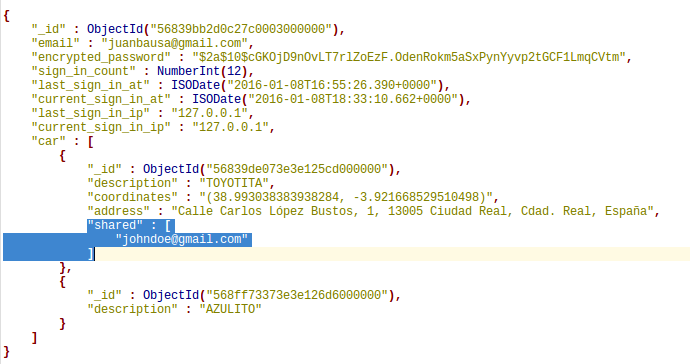
\includegraphics[width=15cm, fbox={\fboxrule} 4mm]{images/05-resultados/20-compartir_coche.png}
%		\caption{Documento con elemento \textit{coche} compartido}
%		\label{fig:compartir_coche}
%	\end{figure}

	\begin{lstlisting}[frame = single, language = JSON, caption  = {«Documento con elemento \textit{coche} compartido»}, label = code:compartir_coche]
		
		{ 
		    "_id" : ObjectId("56839bb2d0c27c0003000000"), 
		    "email" : "juanbausa@gmail.com", 
		    "encrypted_password" : "$2a$10$cGKOjD9nOvLT7rlZoEzF.OdenRokm5aSxPynYyvp2tGCF1LmqCVtm", 
		    "sign_in_count" : NumberInt(12), 
		    "last_sign_in_at" : ISODate("2016-01-08T16:55:26.390+0000"), 
		    "current_sign_in_at" : ISODate("2016-01-08T18:33:10.662+0000"), 
		    "last_sign_in_ip" : "127.0.0.1", 
		    "current_sign_in_ip" : "127.0.0.1", 
		    "car" : [
		        {
		            "_id" : ObjectId("56839de073e3e125cd000000"), 
		            "description" : "TOYOTITA", 
		            "coordinates" : "(38.993038383938284, -3.921668529510498)", 
		            "address" : "Calle Carlos López Bustos, 1, 13005 Ciudad Real, Cdad. Real, España", 
		            "shared" : [
		                "janedoe@gmail.com", 
		                "johndoe@gmail.com"
		            ]
		        }, 
		        {
		            "_id" : ObjectId("568ff73373e3e126d6000000"), 
		            "description" : "AZULITO"
		        }
		    ]
		}
		
	\end{lstlisting}
	
	Se modifica la vista \textit{maps} para que el usuario con permisos sobre elementos \textit{coche} de los que no son propietarios pueda verlos distinguiendo inequívocamente aquellos de los que es propietario de aquellos que están compartidos por otro usuario (ver figura \ref{fig:compartir_coche2}).
	Se modifica la vista \textit{maps} para que en el mapa interactivo se observen mediante marcadores los elementos \textit{coche} compartidos con el usuario.
	
	\begin{figure}[H]
		\centering
		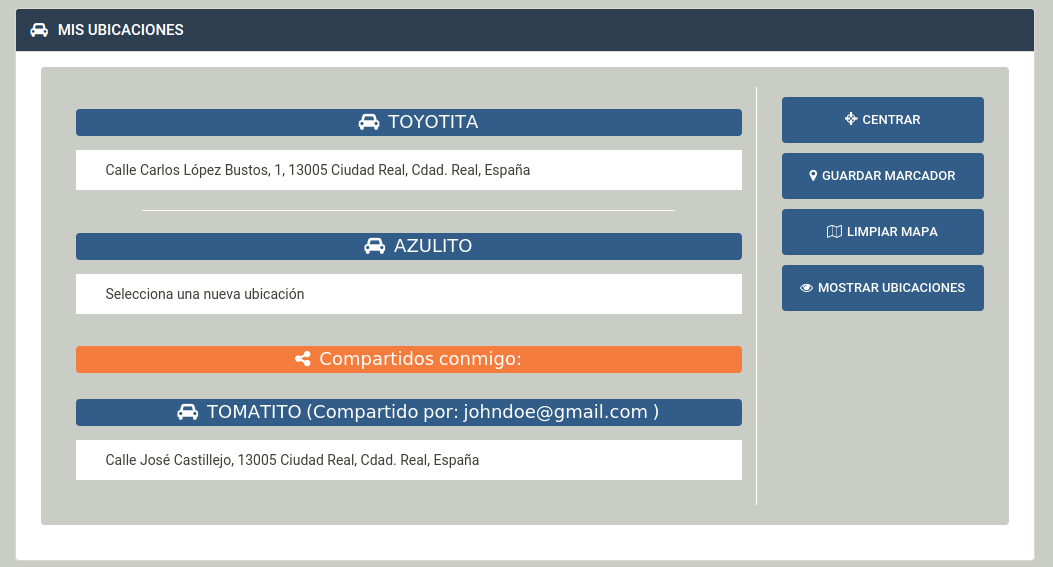
\includegraphics[width=15cm, fbox={\fboxrule} 4mm]{images/05-resultados/21-compartir_coche2.png}
		\caption{Vista con los elementos \textit{coche} compartidos}
		\label{fig:compartir_coche2}
	\end{figure}
	
	Se crea un nuevo campo en el formulario de edición de los elementos \textit{coche}, de tal manera que se puedan añadir los correos electrónicos de los usuarios con los que se quiere compartir el elemento seleccionado. Se crea un nuevo campo en el formulario de edición de los elementos \textit{coche}, de tal manera que se visualiza de manera inequívoca a los usuarios que actualmente mantienen permisos para ver y modificar el elemento seleccionado. Se crea un elemento personalizado en forma de etiqueta que permita detectar con rapidez a los distintos usuarios con permisos sobre el elemento seleccionado (ver figura \ref{fig:compartir_coche3}).
	
	\begin{figure}[H]
		\centering
		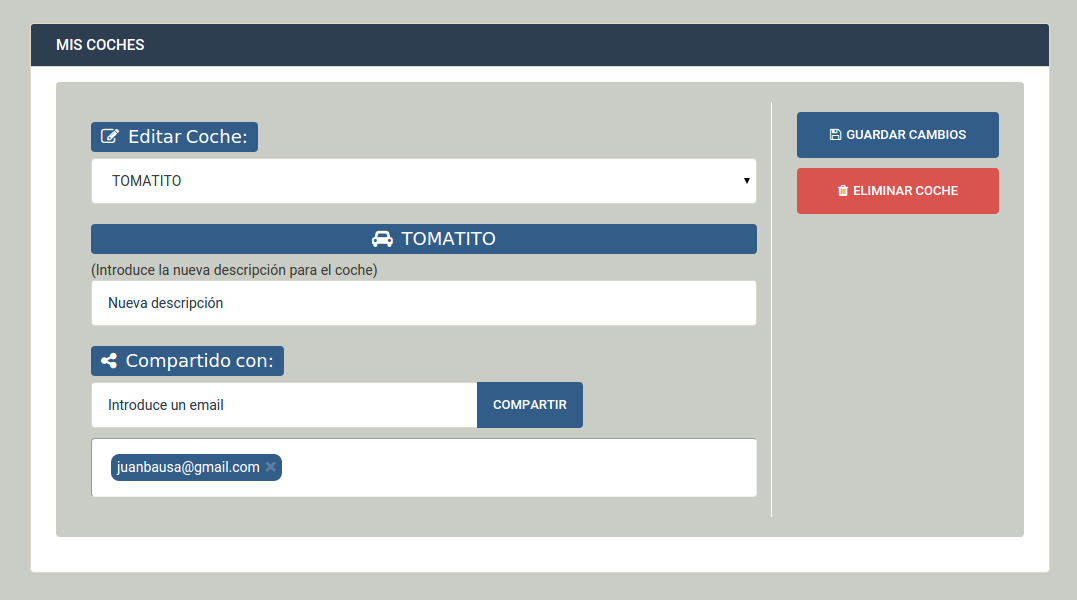
\includegraphics[width=15cm, fbox={\fboxrule} 4mm]{images/05-resultados/22-compartir_coche3.png}
		\caption{Vista de edición elementos \textit{coche} compartidos}
		\label{fig:compartir_coche3}
	\end{figure}	
	
	 Se modifica el controlador de edición de elementos \textit{coche} de manera que incluya la edición de los permisos de compartición.
	 El disparador de la acción continúa siendo el botón creado durante el desarrollo de la historia de usuario 7 en el sprint 4, por lo que únicamente se modifican los parámetros que se envían al controlador.
	 Una vez finalizada la acción, se procede a informar al usuario del resultado de la misma (ver figura \ref{fig:compartir_coche4}).
	 
	 \begin{figure}[H]
		\centering
		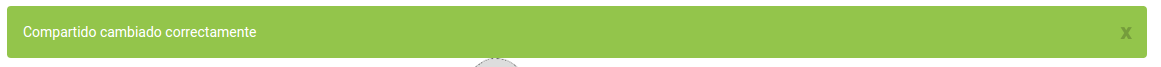
\includegraphics[width=15cm, fbox={\fboxrule} 4mm]{images/05-resultados/23-compartir_coche4.png}
		\caption{Respuesta del controlador}
		\label{fig:compartir_coche4}
	\end{figure}	

	\subsubsection{Desarrollo de la Historia de Usuario: ''Revocar los permisos de acceso a los elementos \textit{coche} del propietario''}	
	Se modifican los elementos personalizados en forma de etiqueta para incluir un nuevo elemento de borrado.
	Se modifica el controlador de edición de elementos \textit{coche} de manera que incluya la revocación de los permisos de compartición.
	El disparador de la acción continúa siendo el botón creado durante el desarrollo de la historia de usuario 7 en el sprint 4, por lo que únicamente se modifican los parámetros que se envían al controlador.
	 Una vez finalizada la acción, se procede a informar al usuario del resultado de la misma.
	
	\subsection{Sprint Review}
	Una vez terminado este sprint, el usuario puede compartir con otros usuarios registrados sus elementos \textit{coche}, de manera que estos últimos pueden ver y editar su posición. También puede revocar los permisos otorgados a estos usuarios.
	
\section{Sprint 8}
	En este sprint se llevará a cabo la historia de usuario 11, consistente en mostrar una ruta a pie desde la ubicación del usuario hasta el elemento \textit{coche} seleccionado.

	\subsection{Refinamiento del Product Backlog}
	No se producen cambios en el \textit{Product Backlog}

	\subsection{Planificación de Sprint}
	Se decide no crear una nueva página de soporte a la funcionalidad, si no reutilizar la página \textit{maps} y la selección de los elementos \textit{coche} para añadir una nueva acción secundaria, de forma que al seleccionar un elemento de la lista, automáticamente aparezcan dibujada la ruta hasta el destino en el mapa.
	
		\begin{table}[H]
	  \centering 
	 	\begin{tabular}{p{0.4\linewidth}p{0.4\linewidth}}
	    \toprule
	    \multicolumn{2}{c}{\cellcolor{black!30}\textbf{Historia de Usuario}} 													\\
		\multicolumn{2}{l}{\cellcolor{gray!25}\textbf{Número: }11}																\\
		\multicolumn{2}{l}{\textbf{Nombre Historia: } Mostrar una ruta a pie hasta el elemento seleccionado}						\\
		\cellcolor{gray!25}\textbf{Valor de negocio: Bajo}	&	\cellcolor{gray!25}\textbf{Riesgo en desarrollo: Bajo}	\\
		\textbf{Esfuerzo:} 6 horas				&	\textbf{Sprint asignado: }8 												\\
		\multicolumn{2}{l}{\cellcolor{gray!25}\textbf{Programador responsable: }Juan Bausá}									\\
		\multicolumn{2}{l}{\textbf{Descripción:}}                                                     						\\
		\multicolumn{2}{l}{\parbox{15cm}{Mostrar la ruta más corta a pie desde la ubicación del usuario hasta el elemento \textit{coche} seleccionado}}				\\
		\multicolumn{2}{l}{\cellcolor{gray!25}\textbf{Resultado:}}																\\		
		\multicolumn{2}{l}{\parbox{15cm}{Al seleccionar un elemento \textit{coche} los usuarios verán dibujada una ruta a pie desde su ubicación hasta dicho elemento.}}																								\\
		\multicolumn{2}{l}{\textbf{Tareas:}}																					\\
		\multicolumn{2}{l}{
			\begin{minipage}{12cm}
	    		\vskip 4pt
	    		\begin{itemize}
	    			\item Modificar el script de generación de los marcadores para incluir una ruta a pie
				\end{itemize}
			  	\vskip 4pt
		 	\end{minipage}
		} \\																				
	    \hline
	  \end{tabular}
	  \caption{Historia de Usuario 10}
	\end{table}
	
	\subsubsection{Desarrollo de la Historia de Usuario: ''Mostrar una ruta a pie hasta el elemento seleccionado''}
	Para el desarrollo de esta nueva funcionalidad, la API de Google Maps nos brinda una forma rápida y sencilla de dibujar la ruta. Únicamente es necesario hacer una llamada a la API pasando como parámetros el punto inicial, es decir, la ubicación actual del usuario y el punto final, la ubicación del elemento seleccionado (ver figura \ref{fig:ruta}).
	
	\begin{figure}[H]
		\centering
		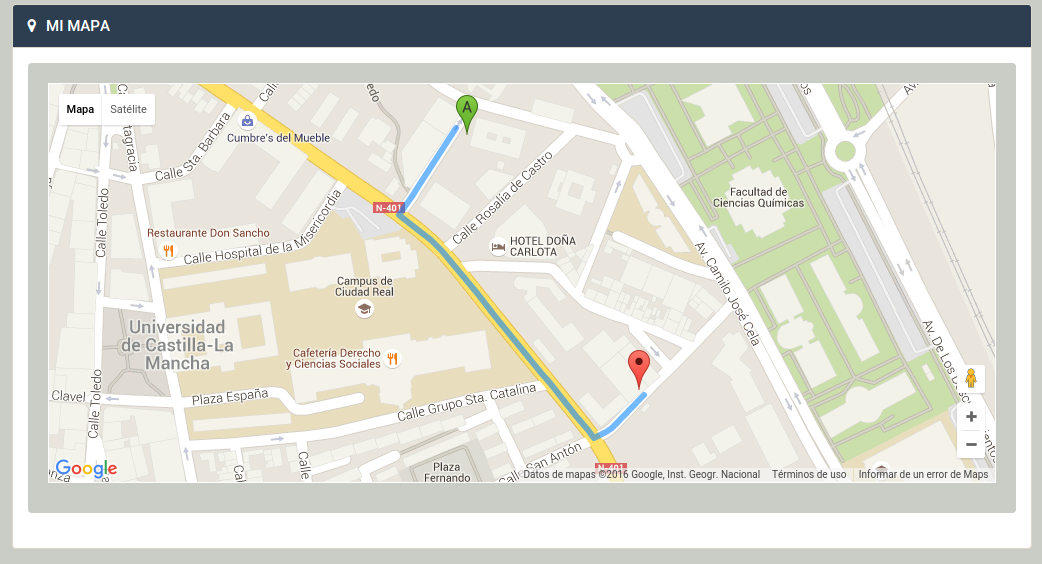
\includegraphics[width=15cm, fbox={\fboxrule} 4mm]{images/05-resultados/24-ruta.png}
		\caption{Vista previa de la ruta a pie}
		\label{fig:ruta}
	\end{figure}
			
	\subsection{Sprint Review}
	Al término de este sprint, cuando el usuario selecciona uno de los elementos \textit{coche} de la lista disponible, se muestra una ruta a pie desde su ubicación detectada y la posición almacenada del elemento.
	
\section{Sprint 9}
En este sprint se llevará a cabo la historia de usuario 12 y el despliegue de la herramienta en el servidor elegido (Heroku).

	\subsection{Refinamiento del Product Backlog}
	Se realizará primero el despliegue en el servidor, debido a que la herramienta móvil quedará configurada con los datos de trabajo finales.

	\subsection{Planificación de Sprint}
	En este último sprint se crea una aplicación móvil que permita el acceso a los usuarios a través de sus dispositivos móviles y se completa el despliegue de la herramienta al servidor elegido durante la fase de planificación, esto es, Heroku.
	
		\begin{table}[H]
	  \centering 
	 	\begin{tabular}{p{0.4\linewidth}p{0.4\linewidth}}
	    \toprule
	    \multicolumn{2}{c}{\cellcolor{black!30}\textbf{Historia de Usuario}} 													\\
		\multicolumn{2}{l}{\cellcolor{gray!25}\textbf{Número: }12}																\\
		\multicolumn{2}{l}{\textbf{Nombre Historia: } Crear una aplicación de acceso para móviles}						\\
		\cellcolor{gray!25}\textbf{Valor de negocio: Bajo}	&	\cellcolor{gray!25}\textbf{Riesgo en desarrollo: Bajo}	\\
		\textbf{Esfuerzo:} 6 horas				&	\textbf{Sprint asignado: }9 												\\
		\multicolumn{2}{l}{\cellcolor{gray!25}\textbf{Programador responsable: }Juan Bausá}									\\
		\multicolumn{2}{l}{\textbf{Descripción:}}                                                     						\\
		\multicolumn{2}{l}{\parbox{15cm}{Crear una aplicación de acceso a la herramienta para móviles Android que permita interactuar al margen de los navegadores instalados en el dispositivo. Despliegue en el servidor elegido.}}				\\
		\multicolumn{2}{l}{\cellcolor{gray!25}\textbf{Resultado:}}																\\		
		\multicolumn{2}{l}{\parbox{15cm}{Los usuarios de dispositivos móviles podrán acceder a la herramienta a través de una aplicación dedicada en sus teléfonos que permitirá el acceso sin necesidad de utilizar los navegadores del dispositivo.}}																								\\
		\multicolumn{2}{l}{\textbf{Tareas:}}																					\\
		\multicolumn{2}{l}{
			\begin{minipage}{12cm}
	    		\vskip 4pt
	    		\begin{itemize}
	    			\item Desplegar el proyecto en el servidor
	    			\item Crear una aplicación móvil
				\end{itemize}
			  	\vskip 4pt
		 	\end{minipage}
		} \\																				
	    \hline
	  \end{tabular}
	  \caption{Historia de Usuario 10}
	\end{table}
	
	\subsubsection{Desarrollo de la Historia de Usuario: ''Crear una aplicación de acceso para móviles''}
La última funcionalidad prevista consiste en implementar una aplicación para móviles que permita el acceso a la página web con la herramienta. Se ha optado por crear una aplicación haciendo uso de la biblioteca \textit{Webview} que permite la carga de páginas web dentro de aplicaciones independendientemente de los navegadores instalados en el sistema.
	
%	\begin{figure}[H]
%		\centering
%		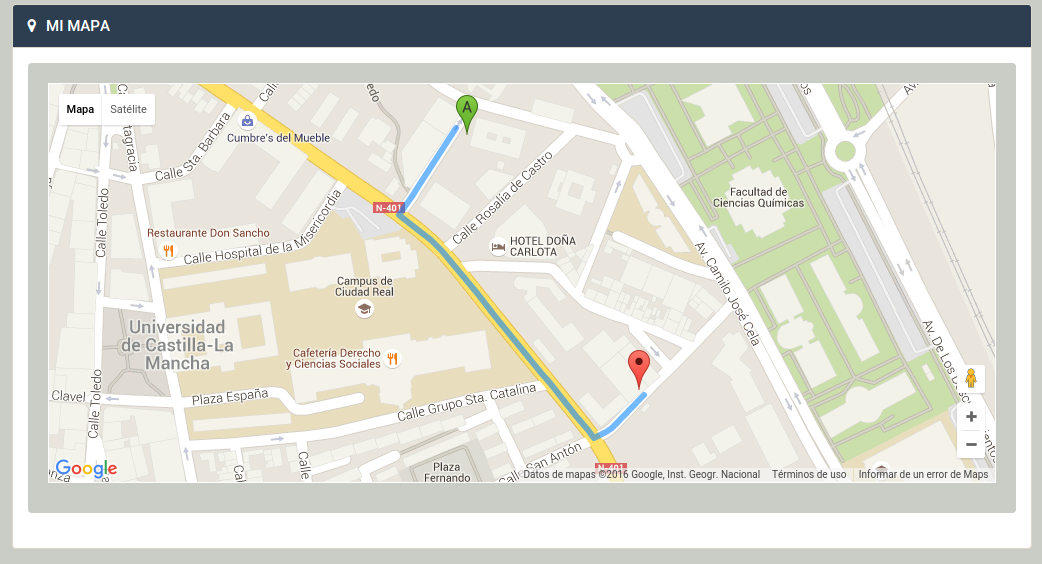
\includegraphics[width=15cm, fbox={\fboxrule} 4mm]{images/05-resultados/24-ruta.png}
%		\caption{Vista previa de la ruta a pie}
%		\label{fig:ruta}
%	\end{figure}
			
	\subsection{Sprint Review}
Con la conclusión de este sprint se considera terminado el desarrollo de la herramienta propuesta.
	
% Local Variables:
%  coding: utf-8
%  mode: latex
%  mode: flyspell
%  ispell-local-dictionary: "castellano8"
% End:
